\documentclass{article}
\usepackage{ctex} % 用于中文支持
\usepackage{geometry}
\geometry{left=3.18cm,right=2.18cm,top=2.54cm,bottom=2.54cm}
\usepackage{graphicx}
\pagestyle{plain}	
\usepackage{setspace}
\usepackage{xcolor}
\usepackage{graphicx}
\usepackage{pdfpages}
\graphicspath{{Figures/}{logo/}} 
\usepackage{fancyhdr}
\renewcommand{\headrulewidth}{0pt} % 去掉页眉的横线
\pagestyle{fancy}

% 清除默认页眉和页脚
\fancyhf{}
% 设置页眉内容
\chead{操作系统实验报告}
\renewcommand{\headrulewidth}{0.5pt}
% 页码
\cfoot{\thepage}
% 设置正文字体大小为5号,

% 宋体
\setCJKmainfont[AutoFakeBold = true, AutoFakeSlant = true]{SimSun}
\setlength{\parindent}{2em} % 段首缩进
\renewcommand{\baselinestretch}{1.5} % 1.5倍行距


\usepackage{listings}
\usepackage{xcolor}
\lstset{
    numbers=left, 
    numberstyle= \tiny, 
    keywordstyle= \color{ blue!70},
    commentstyle= \color{red!50!green!50!blue!50}, 
    frame=shadowbox, % 阴影效果
    rulesepcolor= \color{ red!20!green!20!blue!20} ,
    escapeinside=``, % 英文分号中可写入中文
    xleftmargin=2em, xrightmargin=2em,
    aboveskip=0pt,
    belowskip=0pt,
    framexleftmargin=2em
}





\date{}
\begin{document}
\thispagestyle{empty} % 不显示页码
西安交通大学
	\begin{center}
		\quad \\
		\quad \\
        \vskip 1.5cm
		\heiti \zihao{2} 操作系统专题实验报告
	\end{center}
	\vskip 12cm

	\begin{quotation}
		\songti \fontsize{15}{15}
		\doublespacing
		\par\setlength\parindent{14em}
		\quad 

		班级:\underline{\quad 计算机2101\quad}

		学号:\underline{\quad 2215015058\quad}

		姓名:\underline{\qquad\quad 陈实\qquad }
		\vskip 1cm
		\centering
		2023年12月02日
	\end{quotation}

    \newpage
    \thispagestyle{empty} % 不显示页码
    \tableofcontents

    \thispagestyle{empty}

    \newpage
    \setcounter{page}{1}
    \section{openEuler 系统环境实验}

    \subsection{进程相关编程实验}
    \subsubsection{实验目的}
    \begin{enumerate}
        \item 熟悉 Linux 操作系统的基本环境和操作方法,通过运行系统命令查看
        系统基本信息以了解系统;
        \item 编写并运行简单的进程调度相关程序,体会进程调度、进程间变量的管
        理等机制在操作系统实际运行中的作用。
    \end{enumerate}


    \subsubsection{实验内容}

    \begin{enumerate}
        \item 熟悉操作命令、编辑、编译、运行程序。完成图 1 程序的运行验证,
        多运行几次程序观察结果;去除 wait 后再观察结果并进行理论分析。
        图 1-1 教材中所给代码
        \begin{figure}[htbp]
            \centering
            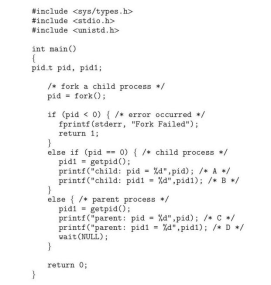
\includegraphics[scale=1.2]{picture/1.png}
            \caption{教材中所给代码(p103 作业 3.7)}
            \label{1}
        \end{figure} 
        \item 扩展图 1 的程序:
        \begin{enumerate}
            \item 添加一个全局变量并在父进程和子进程中对这个变量做不同操作,输出
            操作结果并解释;
            \item 在 return 前增加对全局变量的操作并输出结果,观察并解释;
            \item 修改程序体会在子进程中调用 system 函数和在子进程中调用 exec 族函
            数;
        \end{enumerate}
    \end{enumerate}

    \subsubsection{实验思想}
    
    本实验通过在程序中输出父、子进程的 pid,分析父子进程 pid 之间的关系,
    进一步加入 wait()函数分析其作用。

    \subsubsection{实验步骤}

    \begin{enumerate}
        \item 编写并多次运行图 1-1 中代码
        \item 删去图 1-1 代码中的 wait()函数并多次运行程序,分析运行结果。
        \item 修改图 1-1 中代码,增加一个全局变量并在父子进程中对其进行不同的操作(自行设计),观察并解释所做操作和输出结果
        \item 在步骤三基础上,在 return 前增加对全局变量的操作(自行设计)并输出结果,观察并解释所做操作和输出结果。
        \item 修改图 1-1 程序,在子进程中调用 \texttt{system} 与 \texttt{exec} 族函数。编写 \texttt{system\_call.c} 文件输出进程号 PID,编译后生成 \texttt{system\_call} 可执行文件。在子进程中调用 \texttt{system\_call},观察输出结果并分析总结。
    \end{enumerate}

    \subsubsection{测试数据设计}

    无测试数据

    \subsubsection{程序运行初值及运行结果分析}

    \begin{enumerate}
        \item 编译并运行图 1-1 中代码,运行结果如下:\\
        观察输出,总是先输出子进程的pid,因为有wait(NULL),父进程会等带子进程结束。以第一排输出为例
        在父进程中:\\
        pid: 存放fork()的返回值,也就是子进程的PID。\\
        pid1: 存放getpid()的返回值,也就是父进程自身的PID。\\
        在子进程中:\\
        pid: 存放fork()的返回值0,表示当前是子进程。\\
        pid1: 存放getpid()的返回值,也就是子进程自身的PID。\\
        \newpage
        \begin{figure}[htbp]
            \centering
            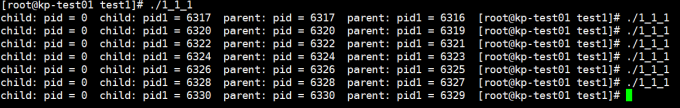
\includegraphics[scale=0.8]{picture/2.png}
            \caption{编译并运行图 1-1 中代码}
            \label{2}
        \end{figure} 
        \item 删去图 1-1 代码中的 wait()函数并多次运行程序\\
        删除wait函数,观察父进程和子进程的输出顺序。输出顺序变化的原因是父进程和子进程的执行顺序不确定,
        取决于系统的调度算法。
        \\
        \begin{figure}[htbp]
            \centering
            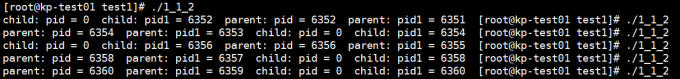
\includegraphics[scale=0.8]{picture/3.png}
            \caption{删去图 1-1 代码中的 wait()函数并多次运行程序}
            \label{3}
        \end{figure} 
        \item 修改图 1-1 中代码,增加一个全局变量并在父子进程中对其进行不同的操作\\
        设置了一个全局变量$value=0$,父进程$value-=100$,子进程$value+=100$,都输出value的值和地址。
        观察父进程和子进程的输出结果。父进程和子进程的value值不同,说明父进程和子进程的数据是独立的,但
        value的地址相同,说明父进程和子进程的地址空间是共享的。
        \begin{figure}[htbp]
            \centering
            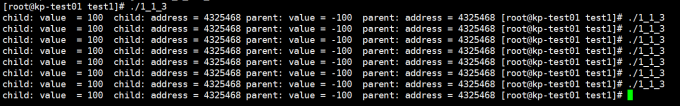
\includegraphics[scale=0.8]{picture/4.png}
            \caption{修改图 1-1 中代码,增加一个全局变量并在父子进程中对其进行不同的操作}
            \label{4}
        \end{figure} 
        \item 在步骤三基础上,在 return 前增加对全局变量的操作(自行设计)并输出结果:\\
        父进程和子进程的value值不同,说明父进程和子进程的数据是独立的,但value的地址相同,说明父进程和子
        进程的地址空间是共享的。

        \newpage
        
        \begin{figure}[htbp]
            \centering
            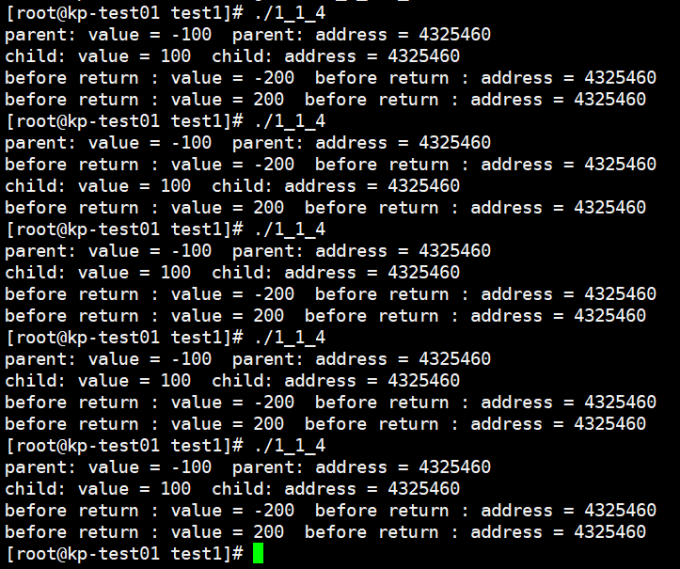
\includegraphics[scale=0.5]{picture/5.png}
            \caption{在步骤三基础上,在 return 前增加对全局变量的操作}
            \label{5}
        \end{figure} 

        \item 修改图 1-1 程序,在子进程中调用 \texttt{system} 与 \texttt{exec} 族函数。
        \texttt{system()}函数:用于在程序中执行另一个可执行文件,与当前进程并行执行\\
        \texttt{exec()} 族函数:用于在程序中执行另一个可执行文件,并将当前进程替换为新的进程
        \begin{figure}[htbp]
            \centering
            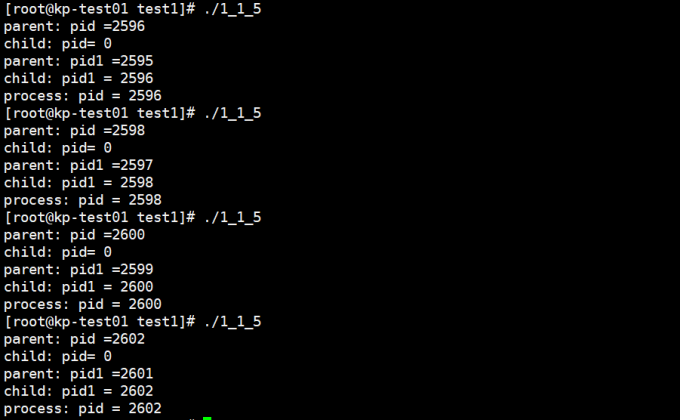
\includegraphics[scale=0.5]{picture/6.png}
            \caption{使用execl函数}
            \label{6}
        \end{figure} 
        以第一次输出为例,子进程的pid为2596,父进程的pid为2595, \texttt{system\_call}的pid为2596,与子进程的pid相同。因为\texttt{execl()}函数会用\texttt{system\_call}可执行文件替换当前进程,所以\texttt{system\_call}的pid与子进程的pid相同。
        \begin{figure}[htbp]
            \centering
            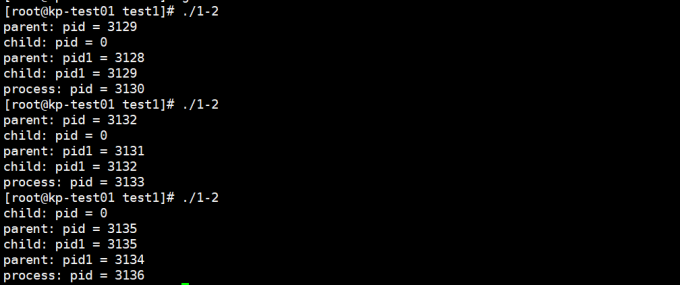
\includegraphics[scale=0.5]{picture/7.png}
            \caption{使用system函数}
            \label{7}
        \end{figure}
        以第一次运行为例, parent的pid为3128, child的pid为3129, \texttt{system\_call}的pid为3130,因为\texttt{system()}函数会新建一个进程,所以\texttt{system\_call}的pid与child的pid不同。
    \end{enumerate}

    \subsection{线程相关编程实验}
    \subsubsection{实验目的}

    \begin{enumerate}
        \item 探究多线程编程中的线程共享进程信息。 在计算机编程中,多线程是一种常
        见的并发编程方式,允许程序在同一进程内创建多个线程,从而实现并发执行。
        由于这些线程共享同一进程的资源,包括内存空间和全局变量,因此可能会出现
        线程共享进程信息的现象。本实验旨在通过创建多个线程并使其共享进程信息,
        以便深入了解线程共享资源时可能出现的问题。
    \end{enumerate}

    \subsubsection{实验内容}

    \begin{enumerate}
        \item 在进程中给一变量赋初值并成功创建两个线程;
        \item 在两个线程中分别对此变量循环五千次以上做不同的操作(自行设计)
        并输出结果;
        \item 多运行几遍程序观察运行结果,如果发现每次运行结果不同,请解释原
        因并修改程序解决,考虑如何控制互斥和同步;
        \item 将任务一中第一个实验调用 system 函数和调用 exec 族函数改成在线
        程中实现,观察运行结果输出进程 PID 与线程 TID 进行比较并说明原因。
    \end{enumerate}


    \subsubsection{实验思想}

    本实验旨在通过创建两个线程,它们分别对一个共享的变量进行多次循环操作,并观察
    在多次运行实验时可能出现的不同结果。在观察到结果不稳定的情况下,引入互斥和同步机制来确保线程间的正确协同操作。

    \subsubsection{实验步骤}

    \begin{enumerate}
        \item 设计程序,创建两个子线程, 两线程分别对同一个共享变量多次操
        作,观察输出结果。
        \item 修改程序, 定义信号量 signal,使用 PV 操作实现共享变量的访问
        与互斥。运行程序,观察最终共享变量的值。
        \item 在第一部分实验了解了 system()与 exec 族函数的基础上,将这两
        个函数的调用改为在线程中实现,输出进程 PID 和线程的 TID 进行分析。
    \end{enumerate}

    \subsubsection{测试数据设计}

    定义共享变量初始值为 0,两个线程分别对其进行100000 次+/- 100 操作,最终在主进程中输出处理后的变量值需要操作次数大才能体现出明显区别

    \subsubsection{程序运行初值及运行结果分析}

    \begin{enumerate}
        \item 设计程序,创建两个子线程, 两线程分别对同一个共享变量多次操作,观察输出结果
        \\由于两个线程没有处理共享变量的同步问题,由于两个线程对sharedVariable的操作是并发的,会同时去操作共
        享变量,所以最后的结果不确定。
        \begin{figure}[htbp]
            \centering
            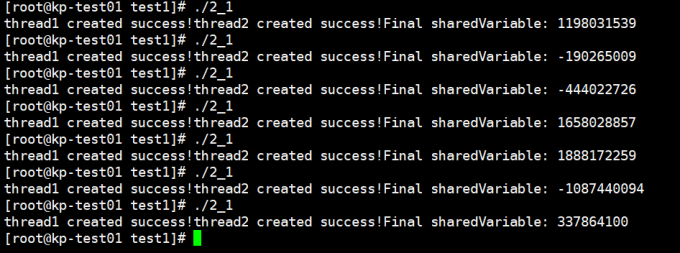
\includegraphics[scale=0.6]{picture/8.png}
            \caption{编译并运行图 1-1 中代码}
            \label{8}
        \end{figure} 

        \item 修改程序, 定义信号量 signal,使用 PV 操作实现共享变量的访问与互斥。运行程序,观察最终共享变量的值。
        \\相较于步骤1,添加了信号量semaphore。 sem\_wait()函数会对信号量semaphore进行P操作, sem\_post()函数会
        对信号量semaphore进行V操作。由于sem\_wait()和sem\_post()函数是原子操作,所以最后的结果为0。由于sem\_wait()和sem\_post()函数是原子操作,每次只有一个线程能够对共享变量进行操作,两个线程对操作是
        相反的,所以最后的结果为0。

        \begin{figure}[htbp]
            \centering
            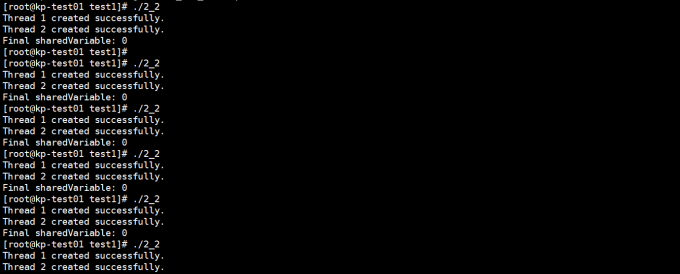
\includegraphics[scale=0.6]{picture/9.png}
            \caption{编译并运行图 1-1 中代码}
            \label{9}
        \end{figure}

        \item 在第一部分实验了解了 system()与 exec 族函数的基础上,将这两个函数的调用改为在线程中实现,输出进程 PID 和线程的 TID 进行分析。\\
        线程1和线程2以及他们调用system\_call2的4个TID都不同,说明线程的TID是独立的。两个线程的PID相同,说
        明两个线程是同一个进程的两个线程。它们调用的system\_call2的PID互不相同且与线程的PID不同,说明调用
        system()函数会新建一个进程。\\
        \begin{figure}[htbp]
            \centering
            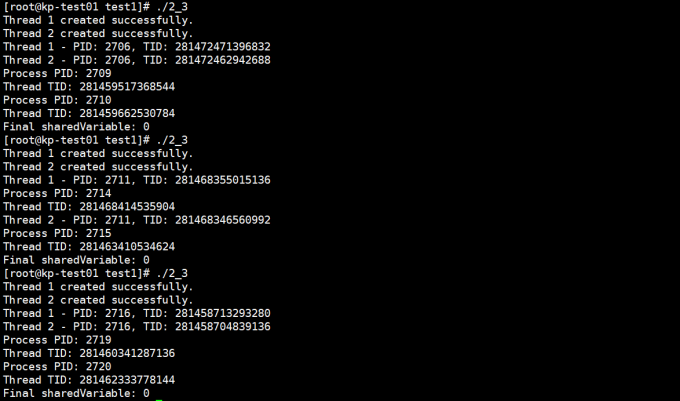
\includegraphics[scale=0.6]{picture/10.png}
            \caption{system函数}
            \label{10}
        \end{figure}
        可以发现只调用成功了一次system\_call2,新的进程的PID与线程的PID相同,说明调用execl()函数会取代当前进
        程。同时,只输出了system\_call2的PID,因为线程属于同一个进程,当一个线程调用execl()函数时,会取代整
        个进程,所以另一个线程的代码不会执行。
        \begin{figure}[htbp]
            \centering
            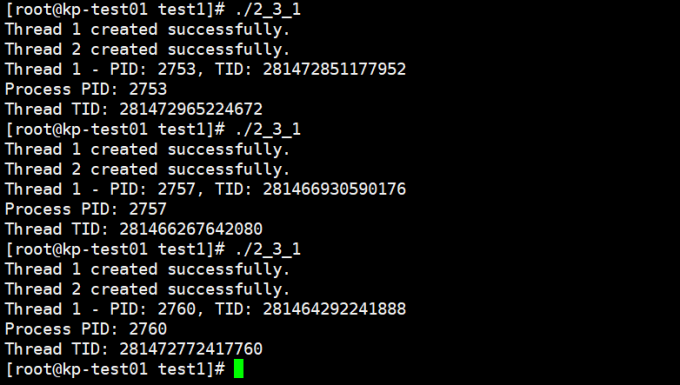
\includegraphics[scale=0.6]{picture/11.png}
            \caption{exec函数}
            \label{11}
        \end{figure}
    \end{enumerate}

    \subsection{自旋锁相关编程实验}
    \subsubsection{实验目的}

    \begin{enumerate}
        \item 了解自旋锁的基本概念: 通过研究自旋锁的工作原理和特点,深入
        理解自旋锁相对于其他锁机制的优势和局限性;
        \item 实验自旋锁的应用: 在一个多线程的实验环境中,设计一个竞争资
        源的场景,让多个线程同时竞争对该资源的访问;
        \item 实现自旋锁的同步: 使用自旋锁来保护竞争资源的访问,确保同一
        时间只有一个线程可以访问该资源,避免数据不一致和竞态条件;
    \end{enumerate}


    \subsubsection{实验内容}


    \begin{enumerate}
        \item 在进程中给一变量赋初值并成功创建两个线程;
        \item 在两个线程中分别对此变量循环五千次以上做不同的操作(自行设计) 并输出结果;
        \item 使用自旋锁实现互斥和同步;
    \end{enumerate}

    \subsubsection{实验思想}
    本实验旨在通过设计一个多线程的实验环境,以及使用自旋锁来实现线程间的同步,

    \subsubsection{实验步骤}

    \begin{enumerate}
        \item 根据实验内容要求,编写模拟自旋锁程序代码 spinlock\.c
        \item 补充完成代码后,编译并运行程序,分析运行结果
    \end{enumerate}


    \subsubsection{测试数据设计}

    无测试数据

    \subsubsection{程序运行初值及运行结果分析}
    由于自旋锁的存在,每次只能有一个线程对共享变量进行操作,所以最后的结果为10000。\\
    在代码实现中是使用了互斥锁,当一个线程对共享变量进行操作时,会对互斥锁进行加锁,其他线程对共享变量进行操作时,会对互斥锁进行加锁,但是加锁失败,所以会一直循环等待,直到加锁成功。\\
        \begin{figure}[htbp]
            \centering
            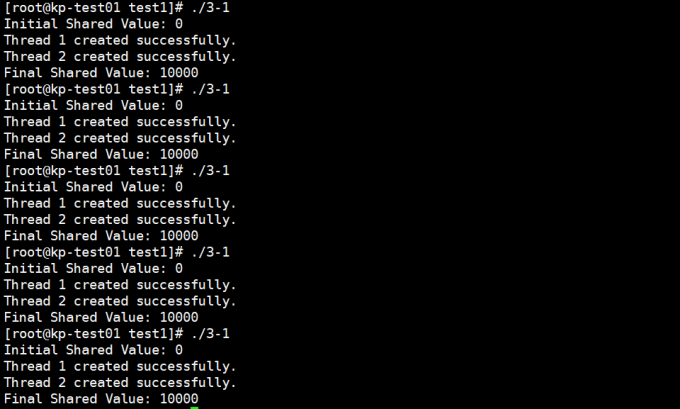
\includegraphics[scale=0.6]{picture/12.png}
            \caption{自旋锁}
            \label{12}
        \end{figure}

    \subsection{实验总结}
    \subsubsection{实验中的问题与解决过程}
    \begin{enumerate}
        \item Linux系统中的输出缓存区的输出与Windows系统的不同,通过查询资料,在Linux系统中,
        printf并不会马上将数据直接输出到屏幕,而是将输出结果暂存在缓冲中,当缓冲区满、
        刷新缓冲区或程序结束时,缓冲区的内容才会进行输出。
    \end{enumerate} 

    \subsubsection{实验收获}

    \begin{enumerate}
        \item 对进程和线程的理解更加的深刻
        \item 了解了如何在程序中调用其他可执行程序,通过system函数以及execl函数
    \end{enumerate}    


    \subsubsection{意见与建议}

    将常见问题总结添加到实验指导书中


    \newpage
    \subsection{附件}
    \subsubsection{附件1 实验1.1代码}
    \lstset{language=C}
    \begin{lstlisting}
#include<sys/types.h>
#include<stdio.h>
#include<unistd.h>
#include<sys/wait.h>

int main(){
    pid_t pid, pid1;
    pid = fork();
    if (pid < 0){
        fprintf(stderr, "Fork Failed");
        return 1;
    }
    else if (pid == 0){
        pid1 = getpid();
        printf("child: pid = %d", pid);
        printf("child: pid1 = %d", pid1);
    }
    else{
        pid1 = getpid();
        printf("parent: pid = %d", pid);
        printf("parent: pid1 = %d/n", pid1);
        wait(NULL);
    }
    return 0;
}
        \end{lstlisting}
        
    \subsubsection{附件2 实验1.2代码}

    \lstset{language=C}
    \begin{lstlisting}
#include <stdio.h>
#include <pthread.h>

#define NUM_THREADS 2
#define NUM_ITERATIONS 100000

int sharedVariable = 0;

void *threadFunction1(void *arg) {
    printf("thread1 created success!");
    for (int i = 0; i < NUM_ITERATIONS; i++) {
        sharedVariable+=i;
    }
    pthread_exit(NULL);
}

void *threadFunction2(void *arg) {
    printf("thread2 created success!");
    for (int i = 0; i < NUM_ITERATIONS; i++) {
        sharedVariable-=i;
    }
    pthread_exit(NULL);
}

int main() {
    pthread_t threads[NUM_THREADS];

    if (pthread_create(&threads[0], NULL,
                 threadFunction1, NULL) != 0) {
        perror("pthread_create");
        return 1;
    }

    if (pthread_create(&threads[1], NULL, 
                threadFunction2, NULL) != 0) {
        perror("pthread_create");
        return 1;
    }
    for (int i = 0; i < NUM_THREADS; i++) {
        pthread_join(threads[i], NULL);
    }
    printf("Final sharedVariable: %d\n", sharedVariable);

    return 0;
}
        \end{lstlisting}


    \subsubsection{附件3 实验1.3代码}

    \lstset{language=C}
    \begin{lstlisting}
        #include <stdio.h>
#include <pthread.h>

typedef struct {
    int flag;
} spinlock_t;

// 初始化自旋锁
void spinlock_init(spinlock_t *lock) {
    lock->flag = 0;
}

// 获取自旋锁
void spinlock_lock(spinlock_t *lock) {
    while (__sync_lock_test_and_set(&lock->flag, 1)) {
        // 自旋等待
    }
}

// 释放自旋锁
void spinlock_unlock(spinlock_t *lock) {
    __sync_lock_release(&lock->flag);
}

// 共享变量
int shared_value = 0;

// 线程函数
void *thread_function(void *arg) {
    spinlock_t *lock = (spinlock_t *)arg;
    for (int i = 0; i < 5000; ++i) {
        spinlock_lock(lock);
        shared_value++;
        spinlock_unlock(lock);
    }
    return NULL;
}

int main() {
    pthread_t thread1, thread2;
    spinlock_t lock;
    // 初始化自旋锁
    spinlock_init(&lock);
    // 创建两个线程
    pthread_create(&thread1, NULL, thread_function, &lock);
    pthread_create(&thread2, NULL, thread_function, &lock);
    // 等待线程结束
    pthread_join(thread1, NULL);
    pthread_join(thread2, NULL);
    // 输出共享变量的值
    printf("Shared Value: %d\n", shared_value);

    return 0;
}
        \end{lstlisting}

    \subsubsection{附件4 README}
    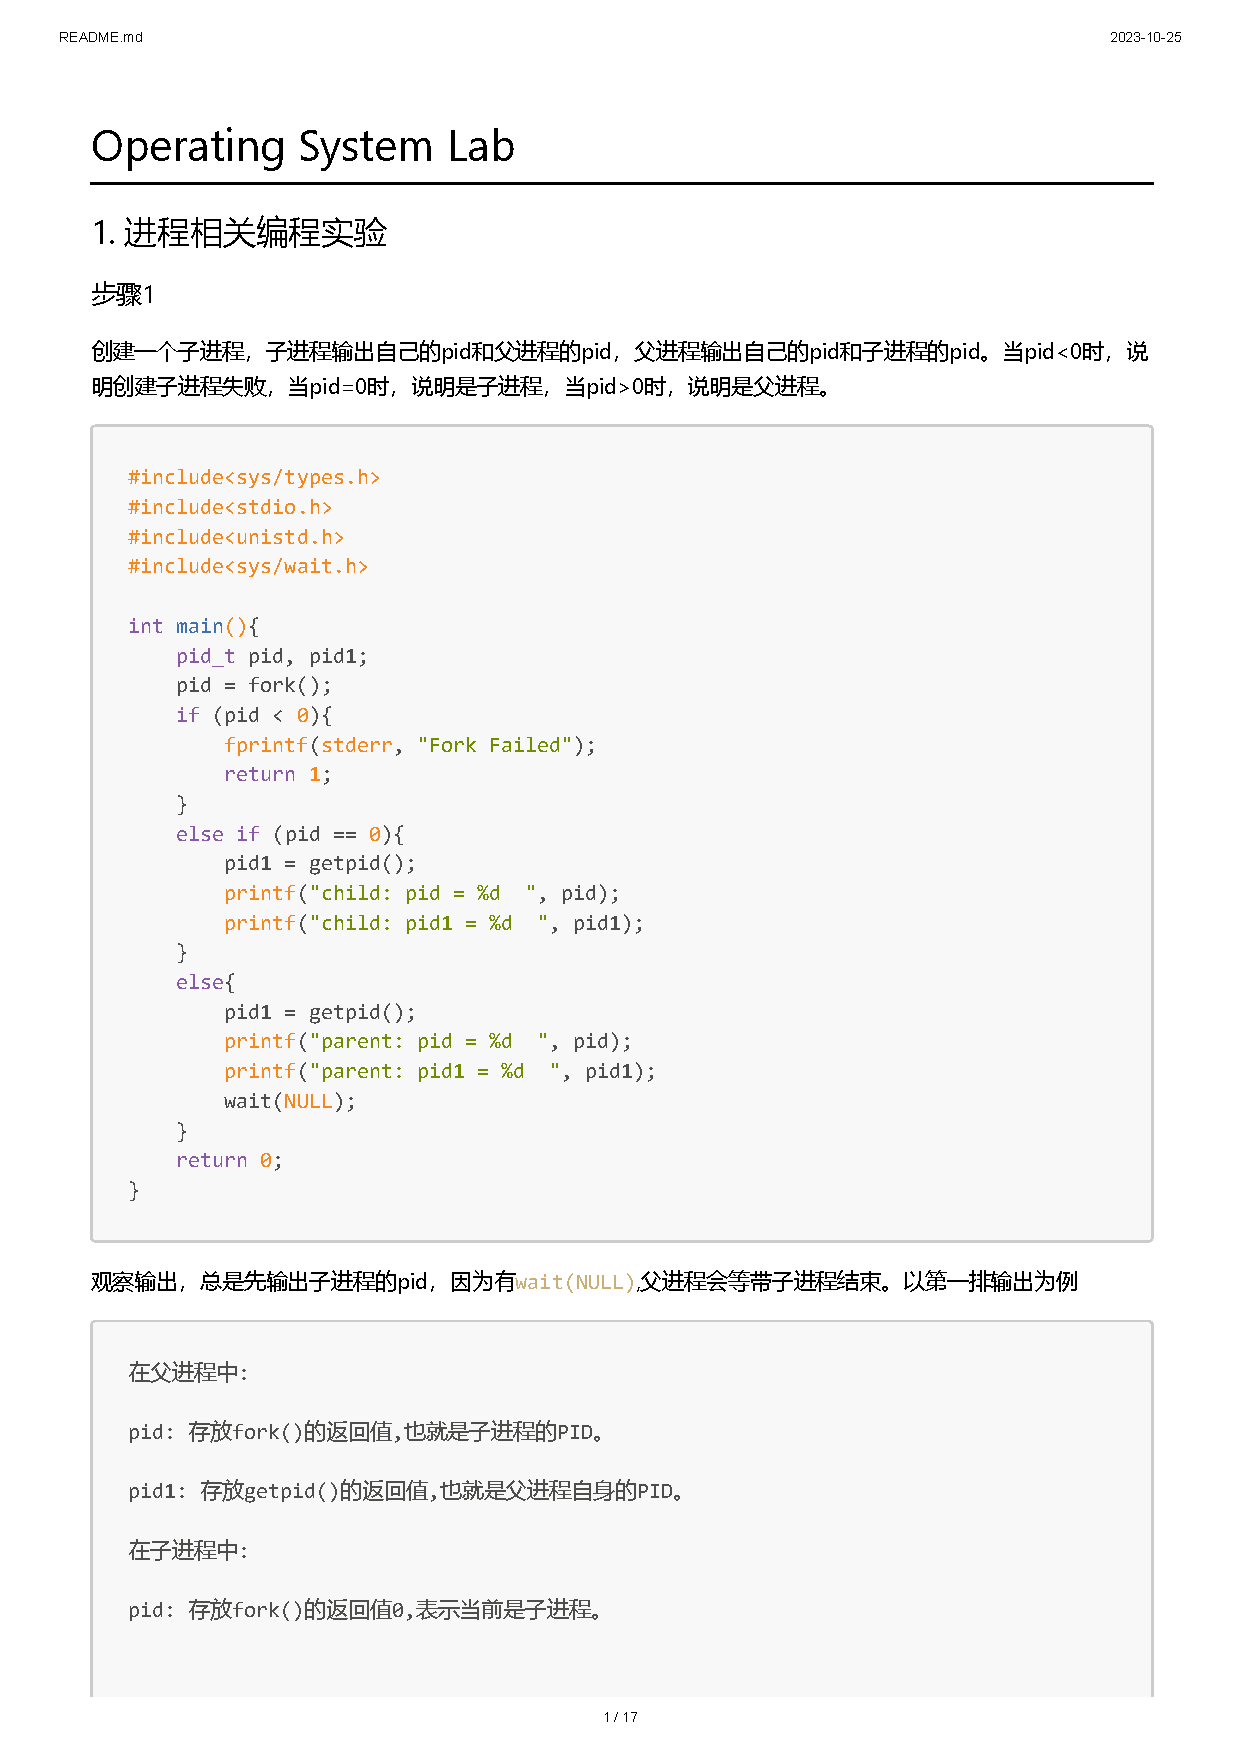
\includepdf[pages=-,scale=.8,pagecommand={}]{1.pdf} 

    \newpage
    \section{进程通信与内存管理}
    \subsection{进程的软中断通信}
    \subsubsection{实验目的}

    \begin{enumerate}
        \item 编程实现进程的创建和软中断通信,通过观察、分析实验现象,深入理解进程及进程在
        调度执行和内存空间等方面的特点,掌握在 POSIX 规范中系统调用的功能和使用。
    \end{enumerate}


    \subsubsection{实验内容}


    \begin{enumerate}
        \item 使用 man 命令查看 fork 、 kill 、 signal、 sleep、 exit 系统调用的帮助手册。
        \item 根据流程图编制实现软中断通信的程序
        \item 多次运行所写程序,比较 5s 内按下 Ctrl+$\backslash$或 Ctrl+Delete 发送中断,或 5s 内不进行
        任何操作发送中断, 分别会出现什么结果?分析原因。
        \item 将本实验中通信产生的中断通过 14 号信号值进行闹钟中断,体会不同中断的执行样
        式,从而对软中断机制有一个更好的理解。
    \end{enumerate}

    \subsubsection{实验思想}

    父进程会从键盘上接收到中断信号,然后向两个子进程分别发出整数值为 16 和 17 软中断信号,
    子进程获得对应软中断信号,执行对应的自定义操作。

    \subsubsection{实验步骤}

    运行三次程序,分别按下 Ctrl+$\backslash$或 Ctrl+Delete 发送中断,或 5s 内不进行任何操作发送中断,观察运行结果。

    \subsubsection{测试数据设计}

    无测试数据

    \subsubsection{程序运行初值及运行结果分析}

    分别测试了5s内按下 Ctrl+$\backslash$或 Ctrl+Delete 发送中断,或 5s 内不进行任何操作发送中断的情况。首先会输出收到的中断信号的值,然后输出子进程收到的中断信号的值,
    子进程获得对应软中断信号,执行对应的自定义操作,printf输出对应提示信息,然后终止子进程。父进程调用 wait()函数等待两个子进程终止后,输出提示信息,结束进程执行。
    \begin{figure}[htbp]
        \centering
        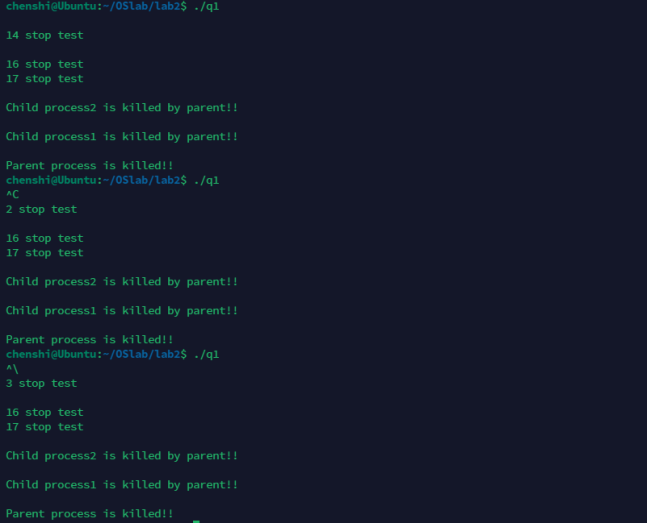
\includegraphics[scale=0.5]{picture/13.png}
        \caption{父进程收到3种不同的中断信号}
        \label{13}
    \end{figure}

    \subsubsection{问题回答}

    \begin{enumerate}
        \item 你最初认为运行结果会怎么样?写出你猜测的结果\\
        父进程收到中断信号后,向两个子进程分别发出整数值为 16 和 17 软中断信号,子进程获得对应软中断信号,执行对应的自定义操作,printf输出对应提示信息。
        \item 实际的结果什么样?有什么特点?在接收不同中断前后有什么差别?请将 5 秒内中断和 5 秒后中断的运行结果截图,试对产生该现象的原因进行分析。\\
        实际结果与预期结果一致。两个子进程输出的顺序不确定。接收不同的中断前没有区别,只有printf的中断值不同。接收不同中断后,子进程收到的中断值不同,执行的操作不同。

        \begin{figure}[htbp]
            \centering
            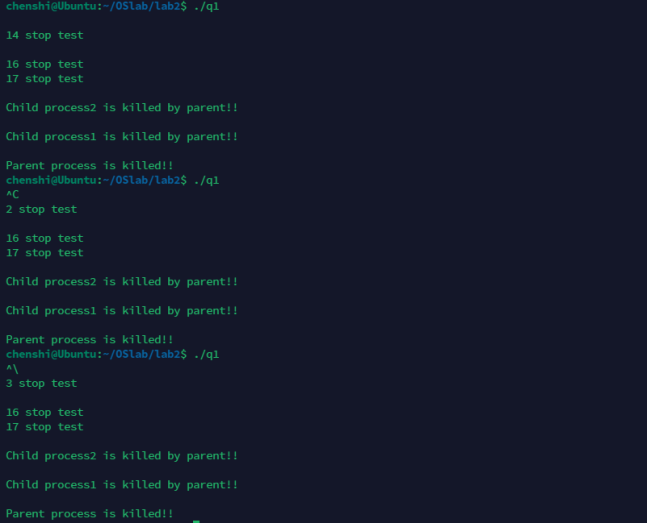
\includegraphics[scale=0.5]{picture/13.png}
            \caption{5s内按下 Ctrl+$\backslash$或 Ctrl+Delete 发送中断}
            \label{14}
        \end{figure}
        产生原因,设置了闹钟中断,5s后会产生闹钟中断。

        \item 改为闹钟中断后,程序运行的结果是什么样子? 与之前有什么不同?
        
        没有不同,因为5s后会产生闹钟中断,所以不会有不同。闹钟中断和软中断的执行函数一样。
        \item kill 命令在程序中使用了几次?每次的作用是什么?执行后的现象是什么?\\
        2次,分别kill两个子进程。执行后,子进程终止。
        \item 使用 kill 命令可以在进程的外部杀死进程。进程怎样能主动退出?这两种退出方式
        哪种更好一些?\\
        使用exit()函数可以在进程的内部杀死进程。使用exit()函数更好,因为可以在进程内部进行一些操作。
    \end{enumerate}

    \subsection{进程的管道通信}
    \subsubsection{实验目的}
    编程实现进程的管道通信,通过观察、分析实验现象,深入理解进程管道通信的特点,
掌握管道通信的同步和互斥机制。
    \subsubsection{实验内容}

    \begin{enumerate}
        \item 学习 man 命令的用法,通过它查看管道创建、同步互斥系统调用的在线帮助,并阅读
        参考资料。
        \item 根据流程图(如图 2.2 所示)和所给管道通信程序,按照注释里的要求把代码补充完
        整,运行程序,体会互斥锁的作用,比较有锁和无锁程序的运行结果,分析管道通信是如何
        实现同步与互斥的。
    \end{enumerate}

    \subsubsection{实验思想}
    父进程创建俩个子进程,一个父子管道,其中两个进程各写入 2000 个字符, 分有锁和无锁的情况。分别观察有锁和无锁情况下的写
    入情况。
    \subsubsection{实验步骤}
    
    \begin{enumerate}
        \item 根据流程图和所给管道通信程序,补全程序,要求使用互斥锁实现管道通信的同步与互斥。
        \item 删除互斥锁,运行程序,观察运行结果。
    \end{enumerate}


    \subsubsection{测试数据设计}
    进程1向管道中写入2000个字符1,进程2向管道中写入2000个字符2。
    \subsubsection{程序运行初值及运行结果分析}

    \begin{enumerate}
        \item 有锁的情况下,在这次测试中,进程1先获取到管道的写入权,将管道上锁
        连续写入了2000个字符1,写完后解锁管道,然后进程2获取到管道的写入权,将管道上锁连续写入了2000个字符2,
        \begin{figure}[htbp]
            \centering
            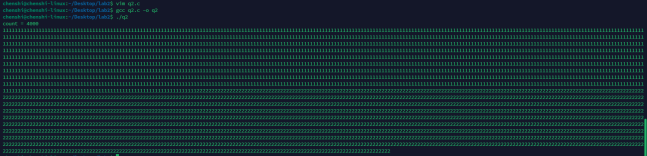
\includegraphics[scale=0.9]{picture/15.png}
            \caption{有锁的情况下}
            \label{15}
        \end{figure}
        \item 无锁的情况下,进程1和进程2争夺管道写入,各写入2000个字符后,进程1和进程2结束。所以在输出中
        \begin{figure}[htbp]
            \centering
            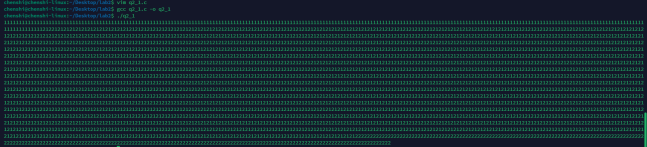
\includegraphics[scale=0.9]{picture/16.png}
            \caption{无锁的情况下}
            \label{16}
        \end{figure}
    \end{enumerate}

    \subsubsection{问题回答}

    \begin{enumerate}
        \item 你最初认为运行结果会怎么样?\\
        有锁的情况下,输出4000个字符,前2000个为同一个字符,后2000个为另一个字符,具体哪个字符在前取决于哪个进程先获取到管道的写入权。\\
        无锁的情况下,4000个字符中字符1和字符2交替混杂出现。
        \item 实际的结果什么样?有什么特点?试对产生该现象的原因进行分析。\\
        实际情况与预测吻合,有锁的情况下,一个进程写入完毕后,另一个进程才能写入。无锁的情况下,两个进程同时写入.
        \item 实验中管道通信是怎样实现同步与互斥的?如果不控制同步与互斥会发生什么后果?\\
        通过对写入段上锁,不上锁输出不可预测
    \end{enumerate}

    \subsection{内存的分配与回收}
    \subsubsection{实验目的}
    通过设计实现内存分配管理的三种算法( FF, BF, WF),理解内存分配及回收的过程及
    实现思路,理解如何提高内存的分配效率和利用率。
    \subsubsection{实验内容}
    
    \begin{enumerate}
        \item 理解内存分配 FF, BF, WF 策略及实现的思路。
        \item 参考给出的代码思路,定义相应的数据结构,实现上述 3 种算法。每种算法要实现内
        存分配、回收、空闲块排序以及合并、紧缩等功能。
    \end{enumerate}

    \subsubsection{实验思想}

    \begin{enumerate}
        \item 首次适应(FF):从内存的起始地址开始查找,找到第一个满足大小要求的空闲分区进行分配。
        \item 最佳适应(BF):从整个空闲分区链表中找到一个最小的满足大小要求的空闲分区进行分配。
        \item 最坏适应(WF):从整个空闲分区链表中找到一个最大的满足大小要求的空闲分区进行分配。
    \end{enumerate}

    \subsubsection{实验步骤}

    \begin{enumerate}
        \item 根据实验内容要求,编写模拟内存分配管理程序代码 memory\.c
        \item 修改程序,实现内存分配管理的三种算法( FF, BF, WF)
        \item 实现内存紧缩
        \item 编译并运行程序,分析运行结果
        \item 比较三种算法的优缺点
    \end{enumerate}

    \subsubsection{测试数据设计}

    \begin{enumerate}
        \item 初始化内存空间,大小为 1024 字节
        \item 分别按FF,BF,WF算法分配内存空间,大小为 100, 200, 300。
        \item 释放内存空间,大小为 200。
        \item 分配内存空间位600,测试内存紧缩
    \end{enumerate}

    \newpage
    \subsubsection{程序运行初值及运行结果分析}

    \begin{enumerate}
        \item  设置内存空间为1024,设置内存分配为Best Fit算法

        
        \begin{figure}[htbp]
            \centering
            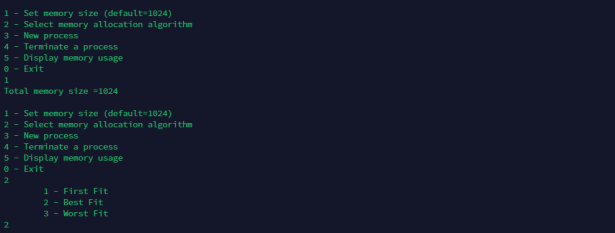
\includegraphics[scale=0.7]{picture/17.png}
            \caption{设置内存空间为1024,设置内存分配为Best Fit算法}
            \label{17}
        \end{figure}
        \item 设置了五个进程,每个进程分配空间为64
        \begin{figure}[htbp]
            \centering
            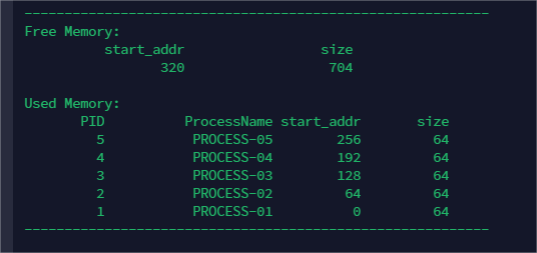
\includegraphics[scale=0.55]{picture/18.png}
            \caption{设置了五个进程,每个进程分配空间为64}
            \label{18}
        \end{figure}
        \item  删除进程2和进程3,展示全部进程的内存分配情况,验证了内存回收的正确性
        \begin{figure}[htbp]
            \centering
            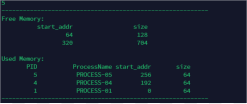
\includegraphics[scale=1.2]{picture/19.png}
            \caption{删除进程2和进程3,展示全部进程的内存分配情况}
            \label{19}
        \end{figure}
        \item 采用worst fit算法,分配一块空间为64的内存,如果实现正确,起始地址应该为320,经
        验证,实现正确

        \begin{figure}[htbp]
            \centering
            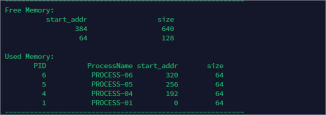
\includegraphics[scale=0.9]{picture/20.png}
            \caption{采用worst fit算法,分配一块空间为64的内存}
            \label{20}
        \end{figure}
        
        \item 采用Best Fit算法,分配一块空间为64的内存,如果实现正确,起始地址应该为64,经
        验证,实现正确

        \begin{figure}[htbp]
            \centering
            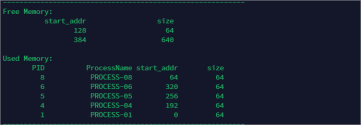
\includegraphics[scale=1]{picture/21.png}
            \caption{采用Best Fit算法,分配一块空间为64的内存}
            \label{21}
        \end{figure}

        \item 采用First Fit算法,分配一块空间为64的内存,如果实现正确,起始地址应该为128,经
        验证,实现正确

        \begin{figure}[htbp]
            \centering
            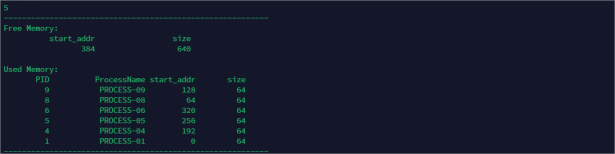
\includegraphics[scale=0.6]{picture/22.png}
            \caption{采用First Fit算法,分配一块空间为64的内存}
            \label{22}
        \end{figure}

        \item 验证内存紧缩的正确性,设置内存为1000,分配五个进程各占用200,释放进程1,3
        \newpage
        \begin{figure}[htbp]
            \centering
            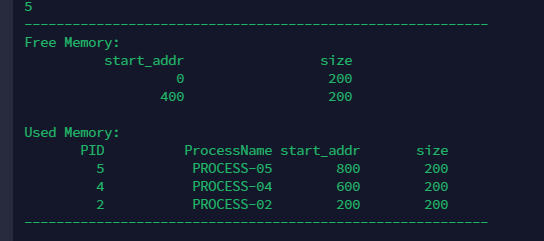
\includegraphics[scale=0.8]{picture/23.png}
            \caption{验证内存紧缩的正确性}
            \label{23}
        \end{figure}

        \item 再新建进程6,分配300内存,会触发内存紧缩,释放所有空闲块,重新分配内存
        
        \begin{figure}[htbp]
            \centering
            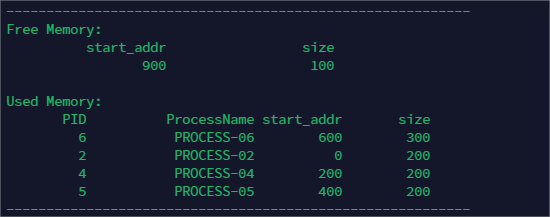
\includegraphics[scale=0.8]{picture/24.png}
            \caption{再新建进程6,分配300内存,会触发内存紧缩}
            \label{24}
        \end{figure}
    
    \end{enumerate}
    \subsubsection{问题回答}

    \begin{enumerate}
        \item 对涉及的 3 个算法进行比较,包括算法思想、算法的优缺点、在实现上如何提高算法
        的查找性能。

        \begin{enumerate}
            \item 算法思想
            \begin{enumerate}
                \item First Fit算法:从内存的起始地址开始查找,找到第一个满足大小要求的空闲分区进行分配。
                \item Best Fit算法:从整个空闲分区链表中找到一个最小的满足大小要求的空闲分区进行分配。
                \item Worst Fit算法:从整个空闲分区链表中找到一个最大的满足大小要求的空闲分区进行分配。
            \end{enumerate}
            \item 算法的优缺点
            \begin{enumerate}
                \item First Fit算法:分配速度快,但是会产生大量的内存碎片。
                \item Best Fit算法:分配速度慢,但是会产生最小的内存碎片。
                \item Worst Fit算法:分配速度慢,但是会产生最大的内存碎片。
            \end{enumerate}

            \item 在实现上如何提高算法的查找性能
            \begin{enumerate}
                \item First Fit算法: 将空闲块按照地址排序,每次分配时从头开始查找,找到第一个满足大小要求的空闲分区进行分配。
                \item Best Fit算法: 将空闲块按照从小到大排序,每次分配时从头开始查找,找到第一个满足大小要求的空闲分区进行分配。
                \item Worst Fit算法: 将空闲块按照从大到小排序,每次分配时从头开始查找,找到第一个满足大小要求的空闲分区进行分配。 
            \end{enumerate}
        \end{enumerate}


        \item 3 种算法的空闲块排序分别是如何实现的。
        
        对于三种算法,都是将空闲块按照某种顺序排序。所以可全部采用同一种排序算法,我使用的是插入排序算法。对于三个算法,分别按照地址,块大小,块大小排序。


        \item 结合实验,举例说明什么是内碎片、外碎片,紧缩功能解决的是什么碎片。
        
        \begin{enumerate}
            \item 内碎片:分配给进程的内存块比进程所需的内存块大,但是进程只用所需的内存块,多余的内存块不能被其他进程使用,这部分内存块就是内碎片。
            \item 外碎片:由于内存块之间的空闲块太小,不能被其他进程使用,这部分内存块就是外碎片。
            \item 紧缩功能解决的是外碎片。
        \end{enumerate}

        \item 在回收内存时,空闲块合并是如何实现的?
        
        在回收内存时,会将回收的内存块与空闲块链表中的空闲块进行合并,合并的方法是将空闲块链表中的空闲块按照地址排序,然后遍历空闲块链表,如果相邻的两个空闲块地址连续,就将两个空闲块合并。
        然后按照原本的排序方式进行排序。

    \end{enumerate}

    \subsection{实验总结}
    \subsubsection{实验中的问题与解决过程}

    \begin{enumerate}
        \item 不了解键盘信号的相关操作,一个信号会发给所有的进程。
        \item 对链表的操作不熟悉,在实现内存紧缩的时候,对链表的操作出现了问题。解决方法:
        将所有的已占用块移到内存的起始位置,然后将所有的空闲块移到已占用块的后面。
    \end{enumerate}

    \subsubsection{实验收获}

    \begin{enumerate}
        \item 对进程的创建和进程间的通信有了更深的理解。
        \item 对内存的分配和回收有了更深的理解。
        \item 对链表的操作有了更深的理解。
        \item 对信号的相关操作有了更深的理解。
    \end{enumerate}

    \subsubsection{意见与建议}

    优化内存的分配与回收部分提供的代码片段,首先调整一下代码的格式,将函数定义和实现放在了主函数前,同时发现了两个应当补全的函数 find\_pid 和 do\_exit,
    但是在代码中没有找到这两个函数的实现,所以在实验中自己实现了这两个函数。

    \subsection{附件}

    \subsubsection{附件1 实验2.1代码}

    \lstset{language=C}

    \begin{lstlisting}
#include <stdio.h>
#include <unistd.h>
#include <sys/wait.h>
#include <stdlib.h>
#include <signal.h>

int flag = 0;
pid_t pid1 = -1, pid2 = -1;

void inter_handler(int signal) {
        flag++;
        printf("\n%d stop test\n\n",signal);
        if (flag==1&& printf("16 stop test\n")&& 
                    printf("17 stop test\n"))
        {
            kill(pid1, 16);
            kill(pid2, 17);
        }
    }

void vv(){};

void waiting() {
    alarm(5);
}

int main() {
    while (pid1 == -1) pid1 = fork();
    if (pid1 > 0) {
        while (pid2 == -1) pid2 = fork();
        if (pid2 > 0) {
            signal(SIGINT, inter_handler);
            signal(SIGQUIT, inter_handler);
            signal(SIGALRM, inter_handler);
            waiting();
            wait(NULL);
            wait(NULL);
            printf("\nParent process is killed!!\n");
        } else {
            signal(SIGQUIT, SIG_IGN);
            signal(SIGINT, SIG_IGN);
            signal(SIGALRM, SIG_IGN);
            signal(17,vv);
            pause();
            printf("\nChild process2 is killed by parent!!\n");
            return 0;
        }
    } else {
        signal(SIGQUIT, SIG_IGN);
        signal(SIGINT, SIG_IGN);
        signal(SIGALRM, SIG_IGN);
        signal(16,vv);
        pause();
        printf("\nChild process1 is killed by parent!!\n");
        return 0;
    }
    return 0;
}
    \end{lstlisting}

    \subsubsection{附件2 实验2.2代码}

    \lstset{language=C}
    \begin{lstlisting}
#include <unistd.h>
#include <signal.h>
#include <stdio.h>
#include <stdlib.h> 
#include <sys/wait.h>

int pid1, pid2;
int main()
{
    int fd[2];
    char InPipe[8000];
    char c1 = '1', c2 = '2';
    pipe(fd);

    while ((pid1 = fork()) == -1);

    if (pid1 == 0)
    {
        close(fd[0]); // 关闭读管道,子进程 1 不需要读
        lockf(fd[1], 1, 0);
        for (int i = 0; i < 2000; i++) {
            write(fd[1], &c1, 1); // 向管道写入字符 '1'
        }
        sleep(5);
        lockf(fd[1], 0, 0);
        exit(0);
    }
    else
    {
        while ((pid2 = fork()) == -1);

        if (pid2 == 0)
        {
            close(fd[0]); // 关闭读管道,子进程 2 不需要读
            lockf(fd[1], 1, 0);
            for (int i = 0; i < 2000; i++) {
                write(fd[1], &c2, 1); // 向管道写入字符 '2'
            }
            sleep(5);
            lockf(fd[1], 0, 0);
            exit(0);
        }
        else
        {
            close(fd[1]); // 关闭写管道,父进程不需要写

            waitpid(pid1, NULL, 0); // 等待子进程 1 结束
            waitpid(pid2, NULL, 0); // 等待子进程 2 结束

            int count = 0;
            while (read(fd[0], &InPipe[count], 1) > 0) {
                count++;
            }
            InPipe[count] = '\0'; // 加字符串结束符
            printf("count = %d\n", count);
            printf("%s\n", InPipe);
            exit(0);
        }
    }
}

    \end{lstlisting}

    \subsubsection{附件3 实验2.3代码}

    \lstset{language=C}
    \begin{lstlisting}
#include <stdio.h>
#include <stdlib.h>
#include <string.h>
#define PROCESS_NAME_LEN 32   /*进程名长度 */
#define MIN_SLICE 10          /* 最小碎片的大小 */
#define DEFAULT_MEM_SIZE 1024 /* 内存大小 */
#define DEFAULT_MEM_START 0   /* 起始位置 */
/* 内存分配算法 */
#define MA_FF 1
#define MA_BF 2
#define MA_WF 3
int mem_size = DEFAULT_MEM_SIZE; /* 内存大小 */
int ma_algorithm = MA_FF;        /* 当前分配算法 */
static int pid = 0;              /* 初始 pid */
int flag = 0;                    /* 设置内存大小标志 */
/* (1) 主要功能 */
/*
1 - Set memory size (default = 1024)
2 - Select memory allocation algorithm
3 - New process
4 - Terminate a process
5 - Display memory usage
0 - Exit
*/

/*(2) 主要数据结构 */
/* 1) 内存空闲分区的描述 */
/* 描述每一个空闲块的数据结构*/
struct free_block_type
{
    int size;
    int start_addr;
    struct free_block_type *next;
};
/* 指向内存中空闲块链表的首指针 */
struct free_block_type*free_block;

/*2) 描述已分配的内存块 */
/* 每个进程分配到的内存块的描述*/
struct allocated_block
{
    int pid;
    int size;
    int start_addr;
    char process_name[PROCESS_NAME_LEN];
    struct allocated_block *next;
};
/* 进程分配内存块链表的首指针 */
struct allocated_block*allocated_block_head = NULL;

/*初始化空闲块,默认为一块,可以指定大小及起始地址*/
struct free_block_type *init_free_block(int mem_size)
{
    struct free_block_type*fb;
    fb = (struct free_block_type *)malloc
                        (sizeof(struct free_block_type));
    if (fb == NULL)
    {
        printf("No mem\n");
        return NULL;
    }
    fb->size = mem_size;
    fb->start_addr = DEFAULT_MEM_START;
    fb->next = NULL;
    return fb;
}

/*显示菜单*/
void display_menu()
{
    printf("\n");
    printf("1 - Set memory size (default=%d)\n", 
                        DEFAULT_MEM_SIZE);
    printf("2 - Select memory allocation algorithm\n");
    printf("3 - New process\n");
    printf("4 - Terminate a process\n");
    printf("5 - Display memory usage\n");
    printf("0 - Exit\n");
}

/*设置内存的大小*/
int set_mem_size()
{
    int size;
    if (flag != 0)
    { // 防止重复设置
        printf("Cannot set memory size again\n");
        return 0;
    }
    printf("Total memory size =");
    scanf("%d", &size);
    char input;
    while ((input = getchar()) != '\n' && input != EOF)
    {
        // 读入一个字符后清空缓存区,避免\n被读入
        //或者一次输入多个字符
    }
    if (size > 0)
    {
        mem_size = size;
        free_block->size = mem_size;
    }
    flag = 1;
    return 1;
}

// 所有的排序算法都采用插入排序,只需要修改比较的条件即可

/*按 FF 算法重新整理内存空闲块链表*/
void rearrange_FF()
{
    if (free_block == NULL)
        return;
    struct free_block_type *current,*next, *temp;
    current = free_block;
    struct free_block_type*new_head = (struct 
    free_block_type *)malloc(sizeof(struct free_block_type)); 
    // 头结点dummy
    new_head->next = NULL;
    new_head->size = 0;
    new_head->start_addr = -1;
    while (current != NULL)
    {
        next = current->next;
        temp = new_head;
        while (temp->next != NULL)
        {
            if (temp->next->start_addr > current->start_addr)
            {
                break;
            }
            temp = temp->next;
        }
        current->next = temp->next;
        temp->next = current;
        current = next;
    }
    free_block = new_head->next;
    free(new_head);
}

/*按 BF 算法重新整理内存空闲块链表*/
void rearrange_BF()
{
    if (free_block == NULL)
        return;
    struct free_block_type *current,*next, *temp;
    current = free_block;
    struct free_block_type*new_head = 
    (struct free_block_type *)malloc
    (sizeof(struct free_block_type));
    new_head->next = NULL;
    new_head->size = 0;
    new_head->start_addr = -1;
    while (current != NULL)
    {
        next = current->next;
        temp = new_head;
        while (temp->next != NULL)
        {
            if (temp->next->size > current->size)
            {
                break;
            }
            temp = temp->next;
        }
        current->next = temp->next;
        temp->next = current;
        current = next;
    }
    free_block = new_head->next;
    free(new_head);
}

/*按 WF 算法重新整理内存空闲块链表*/
void rearrange_WF()
{
    if (free_block == NULL)
        return;
    struct free_block_type *current,*next, *temp;
    current = free_block;
    struct free_block_type*new_head = 
    (struct free_block_type *)malloc
    (sizeof(struct free_block_type));
    new_head->next = NULL;
    new_head->size = 10000000;
    new_head->start_addr = -1;
    while (current != NULL)
    {
        next = current->next;
        temp = new_head;
        while (temp->next != NULL)
        {
            if (temp->next->size < current->size)
            {
                break;
            }
            temp = temp->next;
        }
        current->next = temp->next;
        temp->next = current;
        current = next;
    }
    free_block = new_head->next;
    free(new_head);
}

/*按指定算法重新整理内存空闲块链表*/
void rearrange(int algorithm)
{
    switch (algorithm)
    {
    case MA_FF:
        rearrange_FF();
        break;
    case MA_BF:
        rearrange_BF();
        break;
    case MA_WF:
        rearrange_WF();
        break;
    }
}

/*设置当前的分配算法 */
void set_algorithm()
{
    int algorithm;
    printf("\t1 - First Fit\n");
    printf("\t2 - Best Fit\n");
    printf("\t3 - Worst Fit\n");
    scanf("%d", &algorithm);
    char input;
    while ((input = getchar()) != '\n' && input != EOF)
    {
        // 读入一个字符后清空缓存区,避免\n被读入
        //或者一次输入多个字符
    }
    if (algorithm >= 1 && algorithm <= 3)
        ma_algorithm = algorithm;
    /* 按指定算法重新排列空闲区链表*/
    rearrange(ma_algorithm);
}

//已分配内存空间按照起始地址排序
void sort_allocated_block(){
    struct allocated_block *current,*next, *temp;
    current = allocated_block_head;
    struct allocated_block*new_head = 
    (struct allocated_block *)malloc
    (sizeof(struct allocated_block));
    new_head->next = NULL;
    new_head->size = 0;
    new_head->start_addr = -1;
    while (current != NULL)
    {
        next = current->next;
        temp = new_head;
        while (temp->next != NULL)
        {
            if (temp->next->start_addr > current->start_addr)
            {
                break;
            }
            temp = temp->next;
        }
        current->next = temp->next;
        temp->next = current;
        current = next;
    }
    allocated_block_head = new_head->next;
    free(new_head);
}

/*分配内存模块*/
int  allocate_mem(struct allocated_block *ab)
{
    struct free_block_type*fbt, *pre;
    int request_size = ab->size;
    fbt = pre = free_block;
    if (free_block == NULL)
    {
        return -1;
    }

    // 根据当前算法在空闲分区链表中搜索合适的空闲分区进行分配
    // 分配时需要考虑多种情况,如分割、合并、内存紧缩等
    // 1. 找到可满足空闲分区且分配后剩余空间足够大,则分割
    // 2. 找到可满足空闲分区且但分配后剩余空间比较小,则一起分配
    // 3. 找不可满足需要的空闲分区但空闲分区之和能满足需要,
    //则采用内存紧缩技术,
    // 进行空闲分区的合并,然后再分配
    // 4. 在成功分配内存后,应保持空闲分区按照相应算法有序
    // 5. 分配成功则返回 1,否则返回 -1
    // 请自行补充实现...

    // 找到第一个满足要求的空闲分区
    while (fbt != NULL)
    {
        if (fbt->size >= request_size)
        {
            break;
        }
        pre = fbt;
        fbt = fbt->next;
    }
    // 没找到,则合并空闲分区后再找
    if (fbt == NULL)
    {
        int rest = 0;
        fbt = free_block;
        while (fbt != NULL) {
            rest += fbt->size;
            fbt = fbt->next;
        
        }
        if(rest < request_size) {
            return -1;
        }else {
            sort_allocated_block();
            struct allocated_block* abt=allocated_block_head;
            int prev=0;
            while(abt!=NULL){
                abt->start_addr=prev;
                prev=prev+abt->size;
                abt=abt->next;
            }
            //释放所有空闲分区
            fbt = free_block->next;
            while (fbt != NULL)
            {
                pre = fbt;
                fbt = fbt->next;
                free(pre);
            }
            free_block->size = mem_size-prev;
            free_block->start_addr = prev;
            free_block->next = NULL;
            
        }
        fbt = free_block;
    }
    // 找到了,分配
    if (fbt->size - request_size > MIN_SLICE)
    {
        ab->start_addr = fbt->start_addr;
        ab->size = request_size;
        fbt->start_addr += request_size;
        fbt->size -= request_size;
    }
    else
    {
        ab->start_addr = fbt->start_addr;
        ab->size = fbt->size;
        if (fbt == free_block)
        {
            free_block = fbt->next;
        }
        else
        {
            pre->next = fbt->next;
        }
        free(fbt);
    }
    return 1;
}

/*创建新的进程,主要是获取内存的申请数量*/
int new_process()
{
    struct allocated_block *ab;
    int size;
    int ret;
    ab = (struct allocated_block *)
    malloc(sizeof(struct allocated_block));
    if (!ab)
        exit(-5);
    ab->next = NULL;
    pid++;
    sprintf(ab->process_name, "PROCESS-%02d", pid);
    ab->pid = pid;
    printf("Memory for %s:", ab->process_name);
    scanf("%d", &size);
    char input;
    while ((input = getchar()) != '\n' && input != EOF)
    {
        // 读入一个字符后清空缓存区,避免\n被读入
        //或者一次输入多个字符
    }
    if (size > 0)
        ab->size = size;
    ret = allocate_mem(ab); /* 从空闲区分配内存,
     ret==1 表示分配 ok*/

    /* 如果此时 allocated_block_head 尚未赋值,则赋值 */
    if ((ret == 1) && (allocated_block_head == NULL))
    {
        allocated_block_head = ab;
        return 1;
    }
    /* 分配成功,将该已分配块的描述插入已分配链表 */
    else if (ret == 1)
    {
        ab->next = allocated_block_head;
        allocated_block_head = ab;
        return 2;
    }
    else if (ret == -1)
    {
        /* 分配不成功 */
        printf("Allocation fail\n");
        free(ab);
        return -1;
    }
    return 3;
}

/*根据pid查找内存块*/
struct allocated_block *find_process(int pid)
{
    struct allocated_block*ab = allocated_block_head;
    while (ab != NULL)
    {
        if (ab->pid == pid)
            break;
        ab = ab->next;
    }
    return ab;
}

/*将 ab 所表示的已分配区归还,并进行可能的合并*/
int free_mem(struct allocated_block *ab)
{
    int algorithm = ma_algorithm;
    struct free_block_type*fbt, *pre,*work;

    // 进行可能的合并,基本策略如下
    // 1. 将新释放的结点插入到空闲分区队列末尾
    // 2. 对空闲链表按照地址有序排列
    // 3. 检查并合并相邻的空闲分区
    // 4. 将空闲链表重新按照当前算法排序
    // 请自行补充...

    //  头插法
    work = (struct free_block_type *)
    malloc(sizeof(struct free_block_type));
    if (work == NULL)
    {
        return -1;
    }

    work->start_addr = ab->start_addr;
    work->size = ab->size;
    work->next = free_block;
    free_block = work;

    rearrange_FF(free_block);
    fbt = free_block;
    while (fbt->next != NULL)
    {
        if (fbt->start_addr + fbt->size == fbt->next->start_addr)
        {
            struct free_block_type *temp = fbt->next;
            fbt->size += fbt->next->size;
            fbt->next = fbt->next->next;
            free(temp);
        }
        else
        {
            fbt = fbt->next;
        }
    }
    rearrange(ma_algorithm);

    return 1;
}

/*释放 ab 数据结构节点*/
int dispose(struct allocated_block *free_ab)
{
    struct allocated_block*pre, *ab;
    if (free_ab == allocated_block_head)
    { /* 如果要释放第一个节点 */
        allocated_block_head = allocated_block_head->next;
        free(free_ab);
        return 1;
    }
    pre = allocated_block_head;
    ab = allocated_block_head->next;
    while (ab != free_ab)
    {
        pre = ab;
        ab = ab->next;
    }
    pre->next = ab->next;
    free(ab);
    return 2;
}

/*删除进程,归还分配的存储空间,并删除描述该进程内存分配的节点*/
void kill_process()
{
    struct allocated_block *ab;
    int pid;
    printf("Kill Process, pid=");
    scanf("%d", &pid);
    char input;
    while ((input = getchar()) != '\n' && input != EOF)
    {
        // 读入一个字符后清空缓存区,避免\n被读入
        //或者一次输入多个字符
    }
    ab = find_process(pid);
    if (ab != NULL)
    {
        free_mem(ab); /* 释放 ab 所表示的分配区 */
        dispose(ab);  /* 释放 ab 数据结构节点 */
    }
}

/*显示当前内存的使用情况,包括空闲区的情况和已经分配的情况*/
int display_mem_usage()
{
    struct free_block_type *fbt = free_block;
    struct allocated_block*ab = allocated_block_head;

    printf("------------------------------
    ----------------------------\n");
    /* 显示空闲区 */
    printf("Free Memory:\n");
    printf("%20s %20s\n", "start_addr", "size");
    while (fbt != NULL)
    {
        printf("%20d %20d\n", fbt->start_addr, fbt->size);
        fbt = fbt->next;
    }

    /* 显示已分配区 */
    printf("\nUsed Memory:\n");
    printf("%10s %20s %10s %10s\n", "PID", 
    "ProcessName", "start_addr", "size");
    while (ab != NULL)
    {
        printf("%10d %20s %10d %10d\n", 
        ab->pid, ab->process_name, ab->start_addr, ab->size);
        ab = ab->next;
    }
    printf("-----------------------------
    -----------------------------\n");
}

/*退出,释放所有链表*/

void do_exit()
{
    struct free_block_type *fbt = free_block;
    struct allocated_block*ab = allocated_block_head;
    while (fbt != NULL)
    {
        free_block = fbt->next;
        free(fbt);
        fbt = free_block;
    }
    while (ab != NULL)
    {
        allocated_block_head = ab->next;
        free(ab);
        ab = allocated_block_head;
    }
}

void tab(char choice)
{
}

int main()
{
    char choice, input;
    pid = 0;
    free_block = init_free_block(mem_size); // 初始化空闲区
    while (1)
    {
        display_menu(); // 显示菜单
        choice = getchar();
        while ((input = getchar()) != '\n' && input != EOF)
        {
            // 读入一个字符后清空缓存区,避免\n被读入
            //或者一次输入多个字符
        }
        switch (choice)
        {
        case '1':
            set_mem_size();
            break; // 设置内存大小
        case '2':
            set_algorithm();
            flag = 1;
            break; // 设置算法
        case '3':
            new_process();
            flag = 1;
            break; // 创建新进程
        case '4':
            kill_process();
            flag = 1;
            break; // 删除进程
        case '5':
            display_mem_usage();
            flag = 1;
            break; // 显示内存使用
        case '0':
            do_exit();
            exit(0);
            /*释放链表并退出*/
        default:
            break;
        }
    }
    return 0;
}

    \end{lstlisting}


    \subsubsection{附件4 README}

    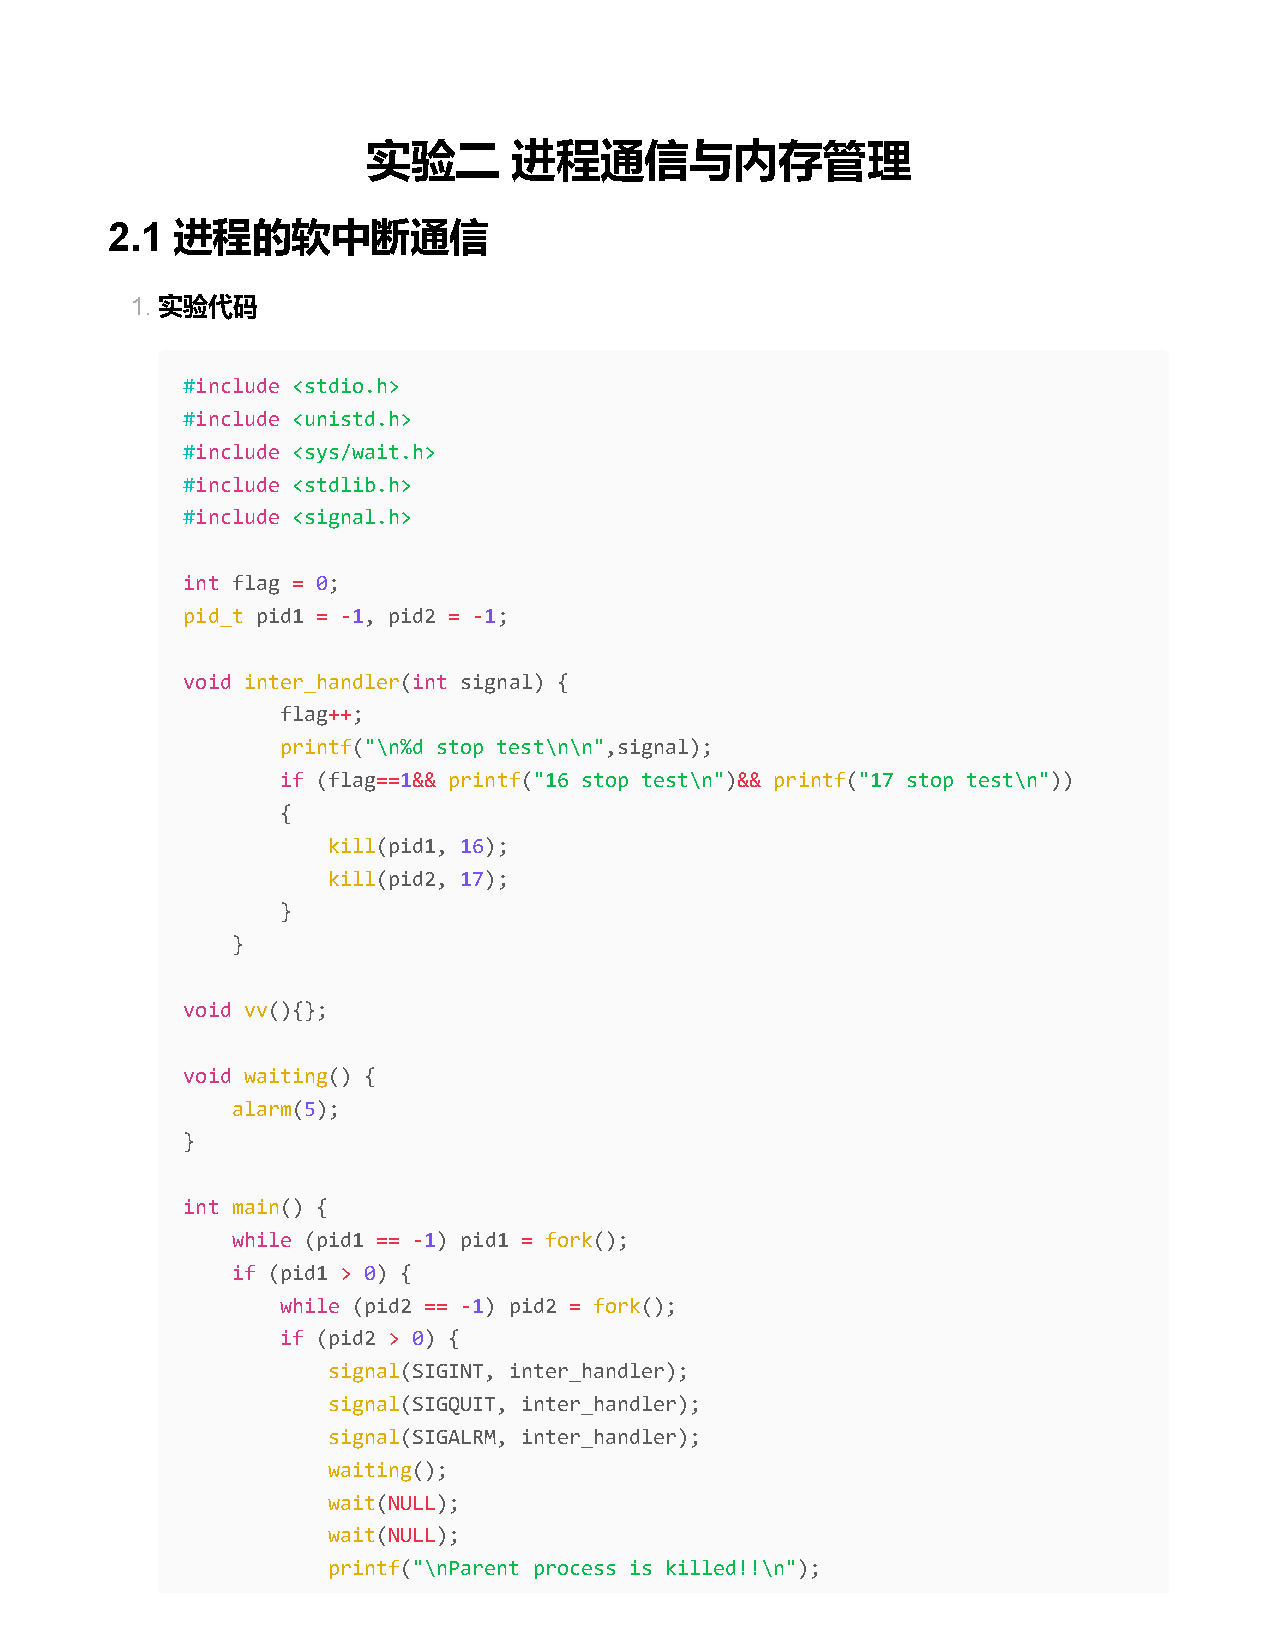
\includepdf[pages=-,scale=.8,pagecommand={}]{2.pdf} 

    \newpage
    \section{文件系统}
    \subsection{实验目的}

    通过一个简单文件系统的设计,加深理解文件系统的内部实现原理


    \subsection{实验内容}

    模拟EXT2文件系统原理设计实现一个类EXT2文件系统

    \subsection{实验思想}

    用一个文件模拟磁盘,用fwrite模仿磁盘的读写操作,用fseek模仿磁盘的寻道操作,用fread模仿磁盘的读操作。

    \subsection{实验步骤}

    \begin{enumerate}
        \item 定义类 EXT2 文件系统所需的数据结构,包括组描述符、索引结点和目录项。
        \item 实现底层函数,包括分配数据块等 操作。
        \item 实现命令层函数,包括 dir 等操作。
        \item 完成 shell 的设计。
        \item 测试整个文件系统的功能。
    \end{enumerate}

    \subsection{测试数据设计}

    \begin{enumerate}
        \item 创建文件系统,格式化磁盘
        \item 在根目录下创建文件夹1
        \item 在文件夹1下创建文件夹2
        \item 在文件夹2下创建文件a
        \item 打开文件a,写入数据
        \item 打开文件a,读出数据
        \item 修改文件a的权限为不可读不可写
        \item 打开文件a,写入数据
        \item 打开文件a,读出数据
        \item 回到根目录,删除文件夹1
    \end{enumerate}

    \subsection{代码简介(具体代码见附件)}

    \begin{enumerate}
        \item 定义类 EXT2 文件系统所需的数据结构,包括组描述符、索引结点和目录项。
        \begin{enumerate}
            \item define部分:定义了一些常量,如磁盘大小、块大小、磁盘起始地址等。
            \item super\_block:超级块,用于存储文件系统的信息,如文件系统名、磁盘总大小、块大小,用户名和密码。
            \item group\_desc:块组描述符,用于存储块位图的起始块号、索引结点位图的起始块号、索引结
            点表的起始块号、本组空闲块的个数、本组空闲索引结点的个数、组中分配给目录的结点
            数。
            \item inode:索引结点,用于存储文件的信息,如文件类型及访问权限、文件所占的数据块个
            数、文件或目录大小、访问时间、创建时间、修改时间、删除时间、直接索引方式 指向数据
            块号。
            \item dir\_entry:目录项,用于存储目录的信息,如索引节点号、目录项长度、文件名长度、文件
            类型、文件名。
            \item 定义了一批全局变量,如最近分配的节点号、最近分配的数据块号、当前目录的节点号、当
            前路径长度、文件打开表、超级块缓冲区、组描述符缓冲区、inode缓冲区、位图缓冲区、
            目录项缓冲区、针对数据块的缓冲区、文件写入缓冲区、虚拟磁盘指针、当前路径名。
            \item 为了方便从文件中读取数据,定义了很多缓冲区,如超级块缓冲区、组描述符缓冲区、
            inode缓冲区、位图缓冲区、目录项缓冲区、针对数据块的缓冲区、文件写入缓冲区。
        \end{enumerate}
        \item 实现底层函数,包括分配数据块等操作。
        \begin{enumerate}
            \item 文件系统各部分的读写\\以超级块为例,通过fopen打开文件,然后通过fseek定位到超级块的位置,再通过fwrite写入
            超级块缓冲区的内容,最后通过fflush立刻将缓冲区的内容输出,保证磁盘内存数据的一致
            性。
            \item 分配数据块与inode节点\\实现思路:记录最近分配的数据块号,然后从这个数据块号开始,从位图循环中寻找空闲的
            数据块,找到后将该数据块置为1,然后更新位图,最后更新组描述符中的空闲块个数
            \item 释放数据块与inode节点\\实现思路:通过位图找到要释放的数据块,然后将该数据块置为0,最后更新组描述符中的
            空闲块个数
            \item 初始化磁盘和文件系统\\初始化磁盘,在当前目录下创建一个名为Ext2的文件,然后将其大小设置为2MB,将各部分
            内容设置为初始化状态,即格式化。\\
            2. 初始化文件系统:读取Ext2文件,然后将各部分内容读取到缓冲区中。
        \end{enumerate}
        \item  命令行函数
        
        \begin{enumerate}
            \item cd命令:切换当前目录,实现思路:通过reserch\_file函数查找目录,然后将当前目录的节点
            号设置为该目录的节点号,最后将当前路径名设置为该目录的路径名。
            \item ls命令:显示当前目录下的文件和目录,实现思路:通过reserch\_file函数查找目录,然后通
            过reload\_dir函数将目录项读取到目录项缓冲区中,最后通过遍历目录项缓冲区,将目录项
            的文件名输出
            \item mkdir命令:创建目录,实现思路:通过reserch\_file函数查找目录,然后通过alloc\_block函
            数分配一个数据块,通过get\_inode函数得到一个inode节点,然后将该目录的信息写入到该
            inode节点中,最后将该目录的信息写入到该数据块中。
            \item touch命令:创建文件,实现思路:通过reserch\_file函数查找目录,然后通过alloc\_block函
            数分配一个数据块,通过get\_inode函数得到一个inode节点,然后将该文件的信息写入到该
            inode节点中。
            \item rm命令:删除文件或目录,实现思路:通过reserch\_file函数查找文件或目录,然后通过
            remove\_block函数释放该文件或目录的数据块,通过remove\_inode函数释放该文件或目录
            的inode节点。
            \item write命令:写文件,实现思路:先通过循环使用getchar函数从键盘读取字符,然后将读取
            到的字符写入到文件写入缓冲区中,知道读取到\#为止,然后根据文件大小,判断是否需要
            使用一级索引或二级索引,最后将文件写入缓冲区中的内容写入到文件中。\\
            为了实现读写保护,在调用write函数时,会先读取该文件对应的inode节点,取i\_mode的倒
            数第二位,如果为1,则说明该文件可写,否则不可写。
            \item  read命令:读文件,实现思路:先通过reserch\_file函数查找文件,然后根据文件大小,判断
            是否需要使用一级索引或二级索引,然后按数据块按字符输出。\\
            为了实行读取保护,在调用读函数后,会先取该文件的inode节点,取i\_mode的倒数第三
            位,只有在为1的时候读出
            \item open命令:打开文件,实现思路:先通过reserch\_file函数查找文件,然后将该文件的inode
            节点号写入到文件打开表中
            \item close命令:关闭文件,实现思路:先通过reserch\_file函数查找文件,然后将该文件的inode
            节点号从文件打开表中删除
            \item chmod命令:修改文件权限,实现思路:通过 i\_mode \& 0x0106 | 0babc 的方式修改文件权
            限.
            \item help命令:显示帮助信息,实现思路:printf输出帮助信息
            \item exit命令:退出文件系统,实现思路:通过exit(0)退出文件系统
            \item format命令:格式化文件系统,实现思路:通过initialize\_disk函数初始化磁盘,然后将各部
            分内容设置为初始化状态,即格式化
        \end{enumerate}
        \item 完成 shell 的设计
        \begin{enumerate}
            \item 模仿Ubuntu的shell,实现思路:通过循环,不断读取用户输入的命令,然后通过strcmp函数
            判断用户输入的命令,然后调用相应的函数。
        \end{enumerate}
    \end{enumerate}

    \subsection{程序运行初值及运行结果分析}

    \begin{enumerate}
        \item 初始化磁盘\\
        初始化磁盘后,设置了Username和Password,然后将其写入到超级块中,然后将各部分内容写入到磁盘中。
        
        \begin{figure}[htbp]
            \centering
            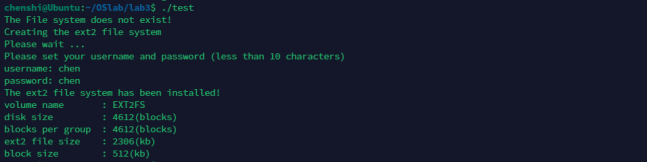
\includegraphics[scale=0.9]{picture/26.png}
            \caption{初始化}
            \label{25}
        \end{figure}

        \item 登录\\
        使用正确的用户名和密码登录,登录成功。使用ls命令查看当前目录下的文件和目录,当前
        目录下有两个目录,分别是 . 和 .. , . 表示当前目录, .. 表示上一级目录。
        默认权限是 r\_w\_\_ ,即可读可写。其中可读指可以cd进入该目录,可写指可以在该目录下创建
        文件或目录。

        \begin{figure}[htbp]
            \centering
            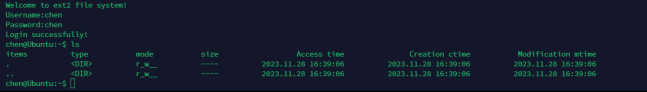
\includegraphics[scale=0.9]{picture/27.png}
            \caption{登录}
            \label{26}
        \end{figure}

        \item 创建目录和文件,写文件\\
        由于a是无后缀的文件,所以默认为有可读可写可执行权限,写入后。使用ls命令查看当前目
        录下的文件和目录,可以看到a文件的大小为30Byte,权限为 r\_w\_x ,Access Time为Open
        的时间,Modify Time为Write的时间,Create Time为Create的时间

        \begin{figure}[htbp]
            \centering
            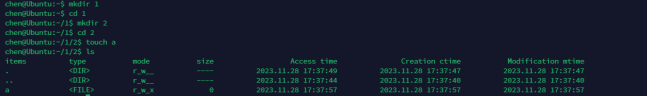
\includegraphics[scale=0.9]{picture/28.png}
            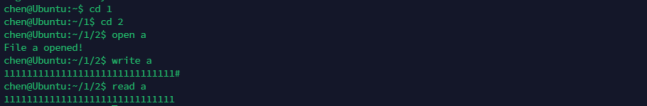
\includegraphics[scale=0.9]{picture/29.png}

        \end{figure}



        \begin{figure}[htbp]
            \centering
            
            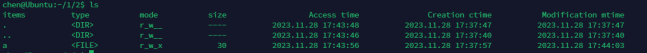
\includegraphics[scale=0.9]{picture/30.png}
            \caption{创建目录和文件,写文件}
            \label{27}
        \end{figure}
        \newpage
        \item 验证读写保护\\
        通过chmod命令修改a文件的权限为 \_\_\_\_x ,即不可读不可写可执行,然后使用read命令读
        取a文件,可以看到读取失败,因为没有读的权限。使用write命令写入a文件,可以看到写入
        失败


        \begin{figure}[htbp]
            \centering
            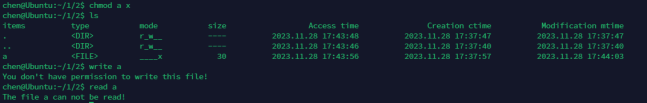
\includegraphics[scale=0.9]{picture/31.png}
            \caption{验证读写保护}
            \label{28}
        \end{figure}

        \item 验证删除多级目录\\
        文件夹1下有文件夹为2,文件夹2下有文件a,然后使用rm命令删除文件夹1,可以看到删除
        成功,验证了删除多级目录的功能。\\
        使用ckdisk命令检查磁盘,可以看到磁盘信息与初始化磁盘时的信息一致,验证了删除多级
        目录后,磁盘信息得到了正确的更新,对应的inode节点和数据块也被释放。

        \begin{figure}[htbp]
            \centering
            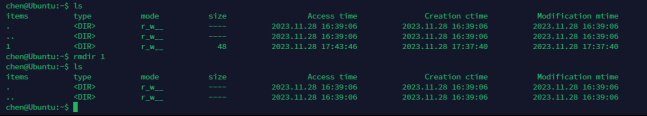
\includegraphics[scale=0.9]{picture/32.png}
            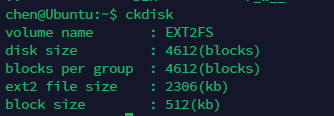
\includegraphics[scale=0.9]{picture/33.png}
            \caption{验证删除多级目录}
            \label{29}
        \end{figure}
    \end{enumerate}

    \subsection{问题回答}

    \begin{enumerate}
        \item 在设计文件系统时数据结构遇到的挑战问题 \\
        在设计文件系统时,遇到的挑战问题是如何将数据结构写入到磁盘中,使用fseek函数定位到对应位置的
        时候会比较复杂,因为需要考虑到各个数据结构的大小,所以需要仔细计算每个数据结构的大小。
        \item 实现底层函数时遇到的挑战问题
        \begin{enumerate}
            \item 实现一级和二级索引的时候,read,write,remove函数都需要适配一级和二级索引。
            \item 频繁的修改要频繁将缓存区写入文件中,偶尔会忘记调用load函数
        \end{enumerate}
        \item 调试代码时遇到的挑战问题\\
        不清楚哪里出错,所以需要仔细检查每个函数的实现,然后通过printf输出调试信息。
    \end{enumerate}

    \subsection{实验总结}
    \subsubsection{实验中的问题与解决过程}
    \begin{enumerate}
        \item 不清楚哪里出错,所以需要仔细检查每个函数的实现,然后通过printf输出调试信息。
        \item 在设计文件系统时,遇到的挑战问题是如何将数据结构写入到磁盘中,使用fseek函数定位到对应位置的
        时候会比较复杂,因为需要考虑到各个数据结构的大小,所以需要仔细计算每个数据结构的大小。
        \item 实现一级和二级索引的时候,read,write,remove函数都需要适配一级和二级索引。
        \item 频繁的修改要频繁将缓存区写入文件中,偶尔会忘记调用load函数
    \end{enumerate}
    \subsubsection{实验收获}

    \begin{enumerate}
        \item 对文件系统的实现有了更深的理解。
        \item 对于c的文件操作更加的熟悉。
        \item 对于大型项目的实现有了更深的理解。
    \end{enumerate}
    \subsubsection{意见与建议}

    延长实验时间,让我们有更多的时间去实现更多的功能。两周的时间实在是太短了。

    \subsection{附件}

    \subsubsection{附件1 ext2\_func.h}

    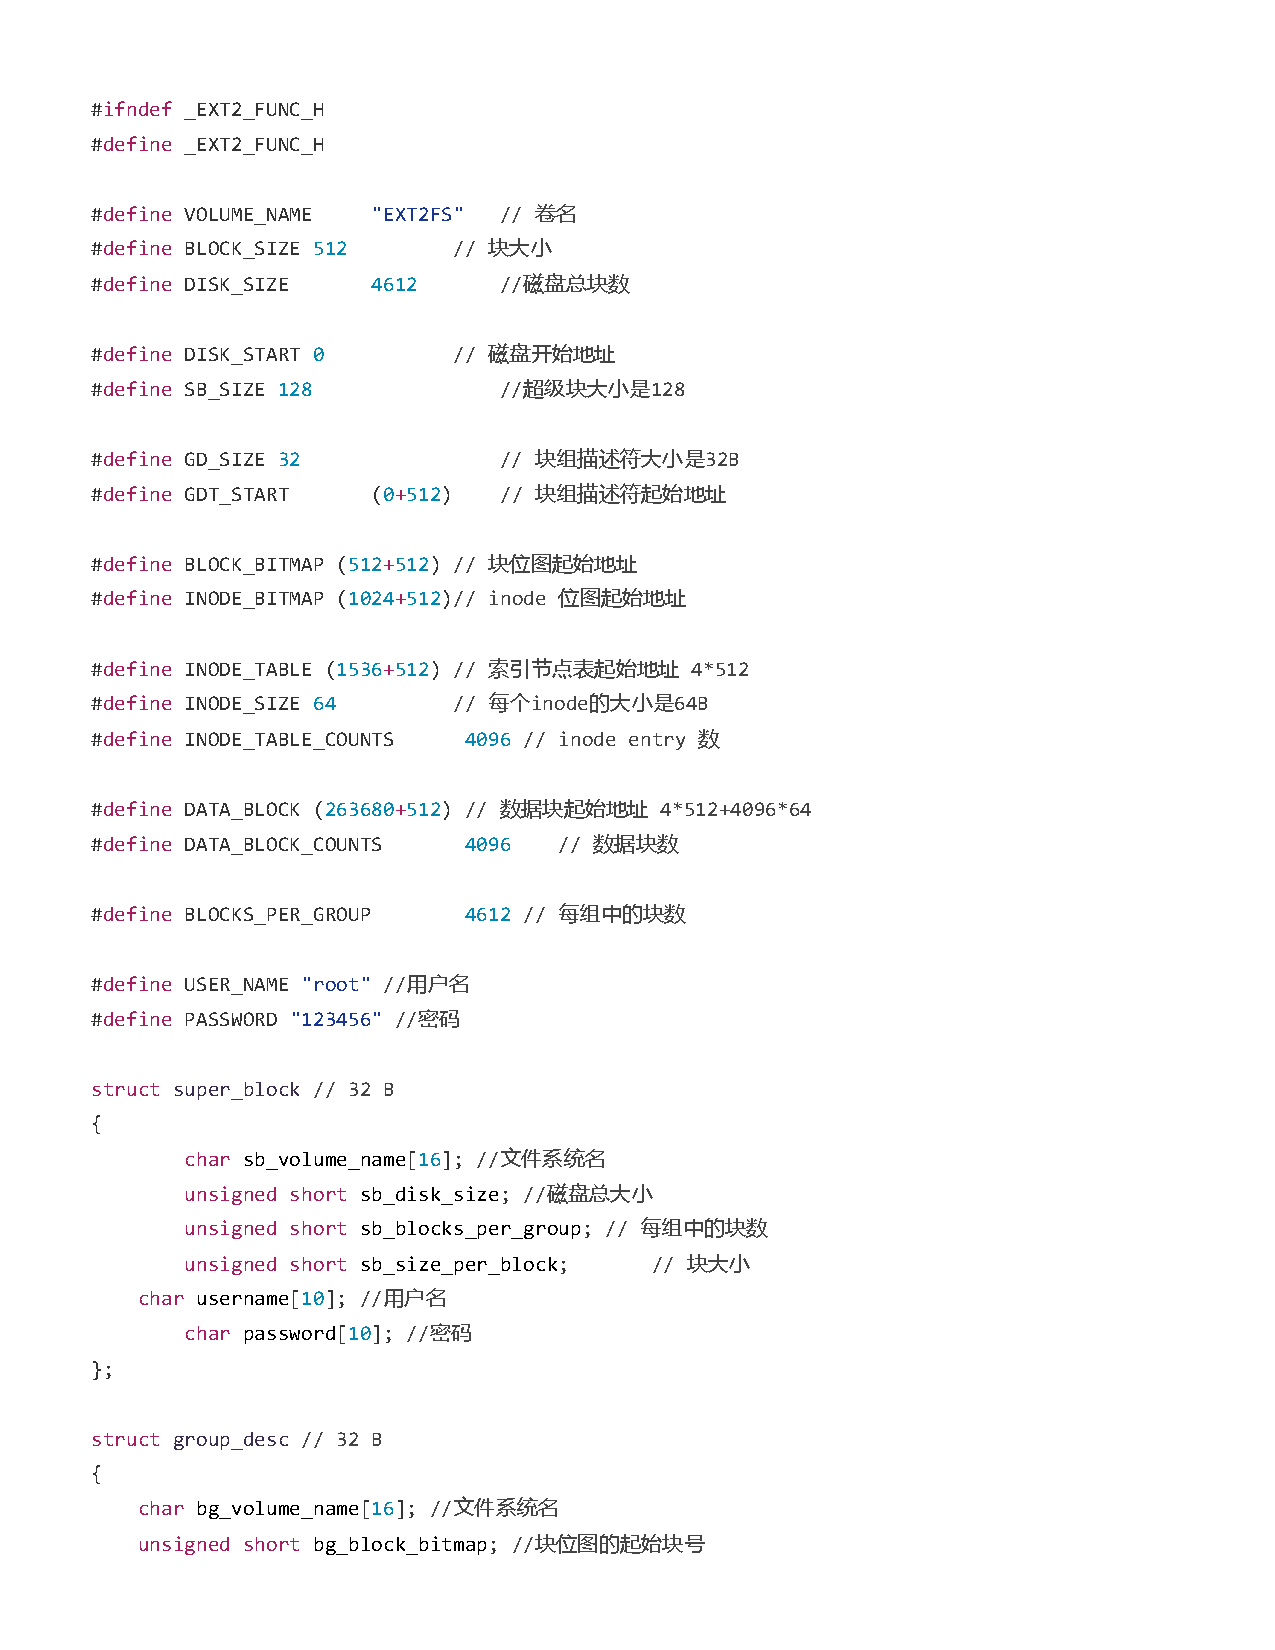
\includepdf[pages=-,scale=.8,pagecommand={}]{3-1.pdf} 
    
    \subsubsection{附件2 ext2\_func.c}

    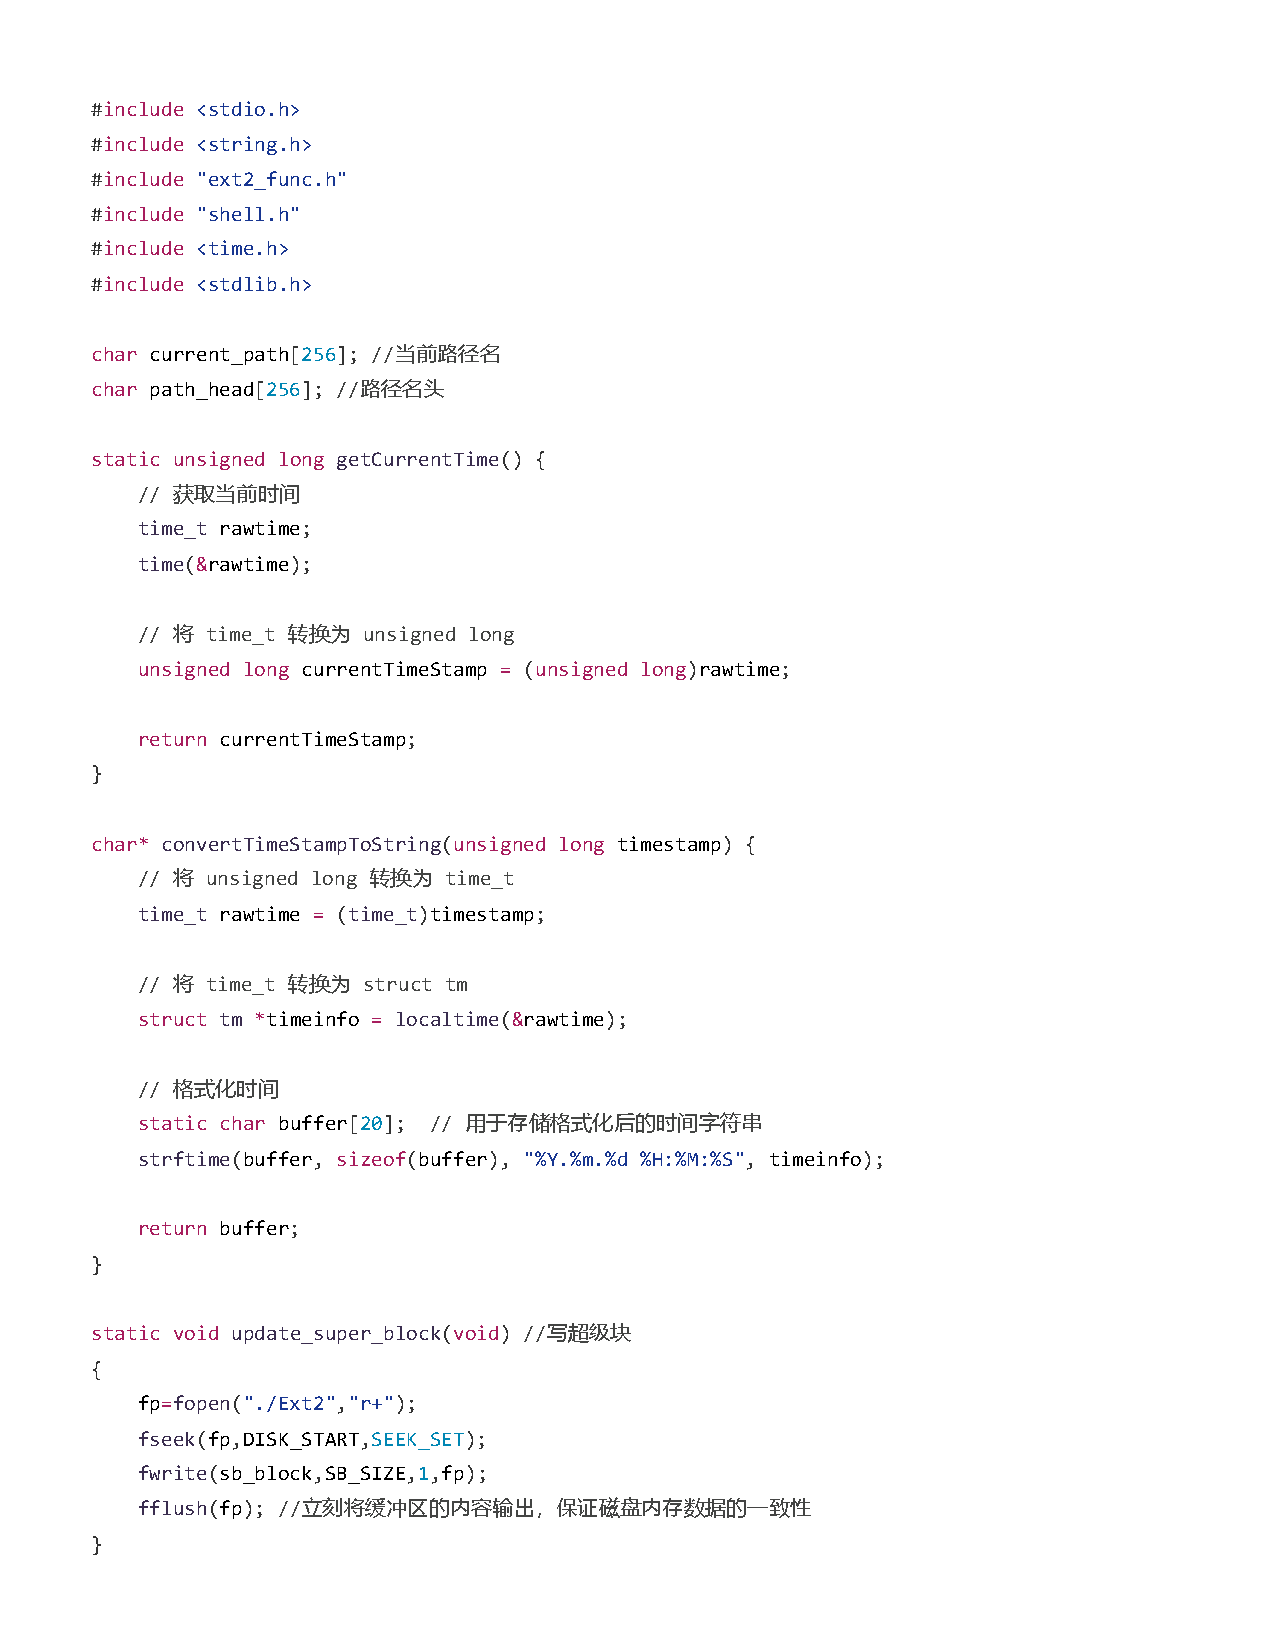
\includepdf[pages=-,scale=.8,pagecommand={}]{3-2.pdf} 
\newpage
    \subsubsection{附件3 shell.h}

    \begin{figure}[htbp]
        \centering
        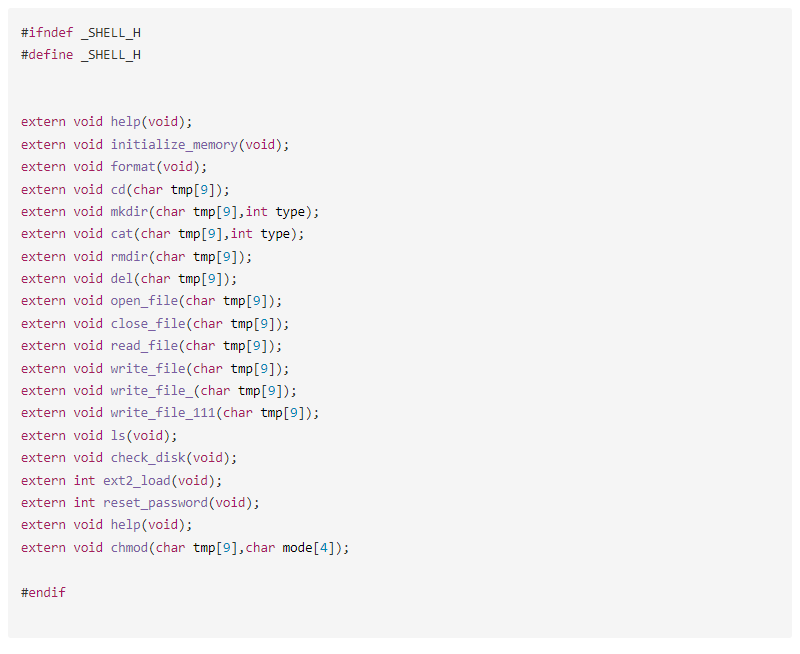
\includegraphics[scale=0.6]{shell_h.png}
        \caption{shell.h}
        \label{30}
    \end{figure}

    \subsubsection{附件4 shell.c}

    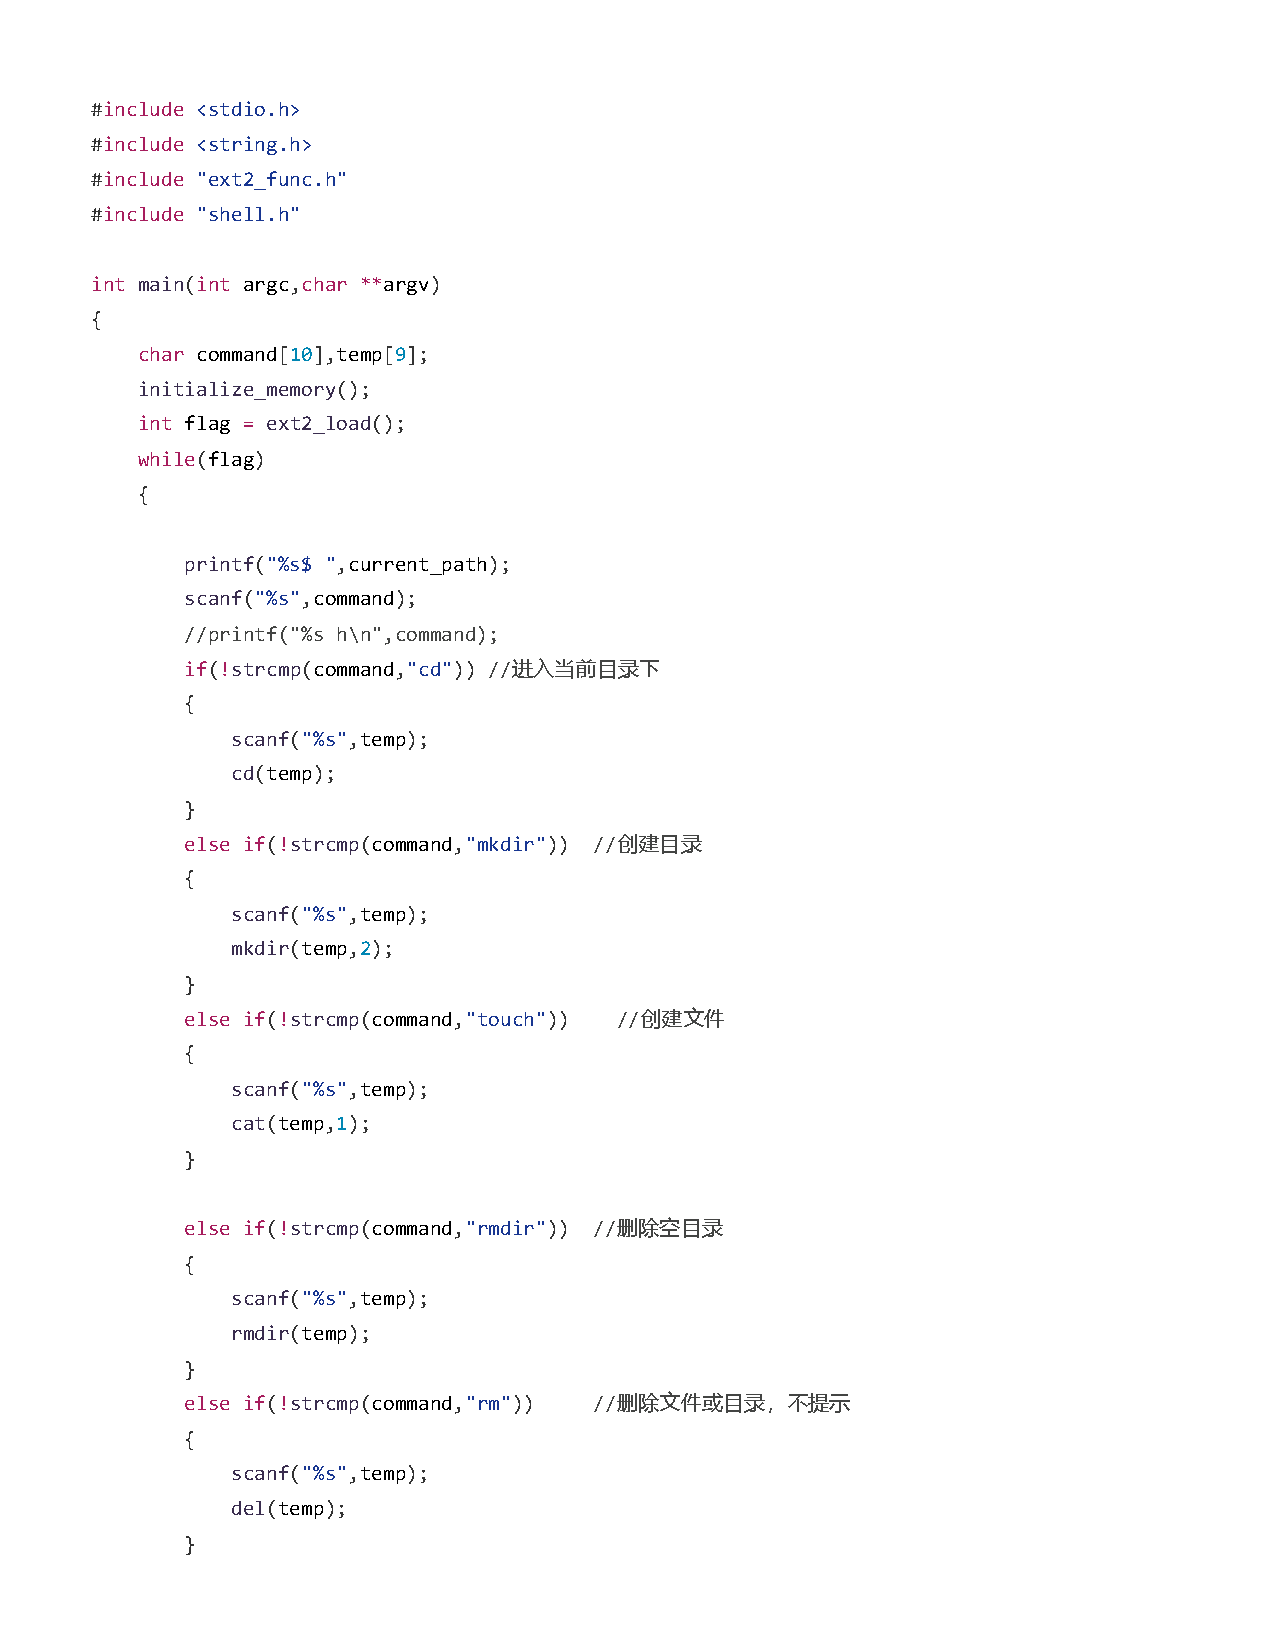
\includepdf[pages=-,scale=.8,pagecommand={}]{3-3.pdf}

    \subsubsection{附件5 README}

    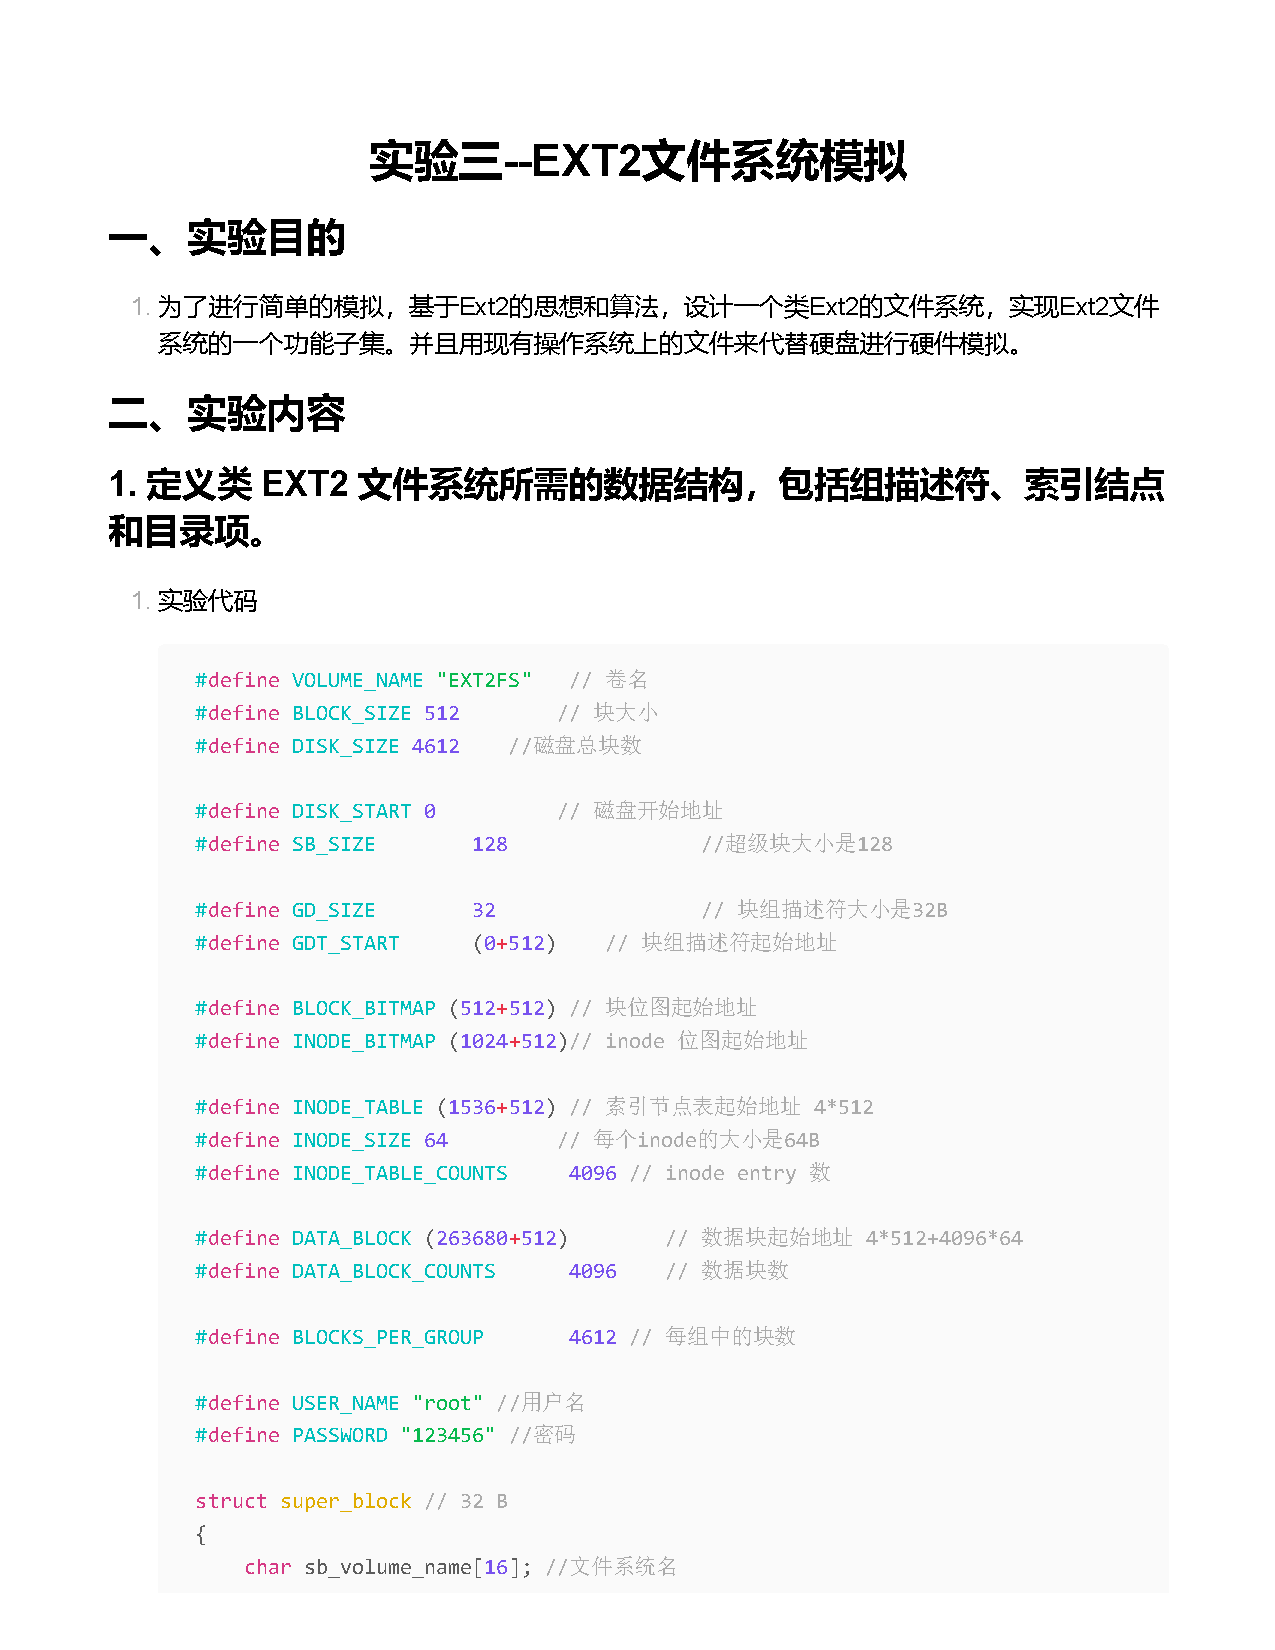
\includepdf[pages=-,scale=.8,pagecommand={}]{3.pdf}

\end{document}